
\chapter{Effect of Grants Restriction on Subnational Governments' Revenue Collection Effort: a Kalman Filter Application}

\section{Introduction}

The relationship between intergovernmental transfers and local governments' tax collection behaviors is pivotal in understanding fiscal dynamics and its consequences on public expenditure patterns. This study investigates whether local governments adjust their tax efforts—either increasing or decreasing them—in response to intergovernmental transfers, and how these adjustments are influenced by any constraints attached to the transfers, such as specific spending requirements. This inquiry is crucial as it affects the overall tax burden within local jurisdictions, potentially influencing population and capital mobility, which may or may not align with federal objectives.
Previous literature primarily examines the relationship between intergovernmental grants amounts and tax collection effort, paying less attention to how spending restrictions attached on these grants influence tax efforts. Within the discussion on the effect of total transfer amounts, the empirical evidence on tax collection efforts remains mixed. Some studies suggest that transfers reduce income disparities, decreasing the need for aggressive tax collection, while others argue for an opposite effect. This discrepancy in findings could stem from two main challenges: a lack of formal theoretical foundation in prior analyses and the difficulty in observing and accurately measuring tax collection efforts.

To address these gaps, this chapter reviews existing literature to outline a comprehensive analytical framework that explicates the underlying mechanisms at play. It utilizes the Kalman filter to refine the measurement of tax collection efforts and conducts a panel data analysis to empirically test the theoretical predictions. The objective is to develop a theoretical model that clarifies the impact of intergovernmental transfers on tax efforts and empirically validate this model, enhancing our understanding of fiscal policy's role in local government behavior.

Chapter 5 represents a pivotal segment of this dissertation by examining the influence of grant restrictions on the revenue collection efforts of subnational governments, thereby addressing a crucial aspect of fiscal federalism—the impact of intergovernmental transfers on local fiscal autonomy and efficiency. This chapter directly ties into the dissertation's broader aim of dissecting the multifaceted interactions between central and subnational governments and their implications for public goods provision and fiscal sustainability. Through the innovative use of a Ramsey model complemented by Kalman filter estimation, this study not only contributes to a deeper theoretical understanding of the mechanisms underpinning fiscal federalism but also offers empirical insights critical for policy formulation. By distinguishing between the effects of general and categorical grants on tax collection efforts, Chapter 5 elucidates the nuanced ways in which different types of intergovernmental transfers can either incentivize or disincentivize local tax effort. This investigation enriches our comprehension of the strategic fiscal behaviors that characterize the relationships within fiscal federalism, thus enhancing the overall narrative of the dissertation by highlighting the importance of grant design in fostering an equitable and efficient provision of public services across government tiers.

The chapter is structured as follows: It begins with an overview of tax effort and its significance to actual tax burdens, followed by a review of the relevant literature. It then details the theoretical model and hypotheses, and employs a panel data model to test these hypotheses, aiming to contribute to a more nuanced understanding of the fiscal interplay between different levels of government.

\section{Background}

The background information section will aim to introduce the concept of tax effort and its relationship with the actual tax burden. It will facilitate the subsequent discussion on whether using the actual tax burden as a measure of tax effort in the existing literature is justified.

The concept of tax effort plays a critical role in fiscal policy analysis, bridging the gap between legal tax rates and the actual tax burden experienced by citizens. Unlike the statutory tax rates, which are often rigid due to legislative processes, tax effort reflects the discretionary practices of subnational governments to manage their revenue collection without altering the legal tax framework. For example, while the United States Congress has the authority to modify federal tax rates, local administrations may employ various strategies, such as offering tax incentives or enforcing different degrees of compliance rigor, to effectively adjust the tax burden on their constituents.

This nuanced approach allows subnational entities to respond to fiscal transfers from higher levels of government and other economic variables without needing formal tax legislation adjustments. Tax effort, therefore, encapsulates the extent to which local governments exploit their tax base, considering the limitations imposed by their administrative and legal frameworks. It encompasses actions like granting tax reliefs, managing exemptions, and varying the intensity of tax collection efforts, all of which affect the actual tax rate applied to the economy.

Understanding the dynamic between tax effort and the actual tax burden is essential for analyzing fiscal policy's impact on economic behavior and public finance. It highlights the importance of administrative discretion in tax collection and the need for analytical models that can accurately capture these subtleties. This paper aims to contribute to this understanding by proposing a theoretical framework and empirical analysis that account for the complexities of tax effort and its determinants, setting the stage for a deeper investigation into how intergovernmental transfers influence these efforts.


\section{Literature Review}

In this section, we delve into the existing literature on the relationship between intergovernmental transfers and tax efforts, aiming to dissect the theoretical perspectives and empirical findings that characterize this field. Our goal is to synthesize the main trends, critical insights, and remaining gaps within this area of study, thereby laying a solid foundation for understanding the current state of research and identifying avenues for future investigation.

Our literature review is structured into two principal segments:

Firstly, we will explore both theoretical and empirical studies that examine the impact of intergovernmental transfers on local government tax efforts. This includes analyses that investigate the potential for transfer payments to substitute for local revenue collection efforts (diminishing tax effort), as well as studies that suggest circumstances under which transfers might encourage the expansion of the tax base. By integrating these bodies of work, we aim to highlight the dominant arguments and findings in the field, noting the congruences and discrepancies between theoretical predictions and empirical observations.

Secondly, we will delve into the specific challenges and issues encountered in empirical research within this domain. This segment will emphasize the key difficulties faced by researchers, such as data constraints, methodological choices, and accurately assessing the effect of intergovernmental transfers on tax efforts. By examining these challenges, we seek to reveal the critical questions that future research must address to deepen our understanding of the dynamics between intergovernmental transfers and tax efforts.

Through this organizational approach, we aspire not only to summarize and critique the significant contributions of the existing literature but also to highlight the direction for our studies. This classification facilitates a clear distinction between theoretical expectations and empirical validations, emphasizing the gaps and challenges present in current research. This sets the stage for the subsequent parts of our study, where we will first thoroughly investigate the theoretical and empirical research on the impact of transfers on tax efforts before turning our attention to the major issues and challenges encountered in empirical stud

\subsection{Theoretical and Empirical Insights on Intergovernmental Transfers and Tax Effort}

Inherent to the nature of general transfer is that transfer would lead to tax fungibility effect, which means transfer would substitute local governments' revenue collection efforts. This phenomenon is also referred to as the crowding out effect on tax effort and has been supported by bunch of evidences \parencite{inman1988federal,peterson1997decentralization,litvack1998rethinking}. Empirical evidence in both developed and developing countries has further confirmed this theoretical inference. For example, Nicholson \cite{nicholson2008fiscal} discovered the fungibility effect of intergovernmental transfer on tax effort at the state level in Germany and the United States.  \textcite{2002A}, \textcite{aragon2005intergovernmental}, \textcite{panda2009central}, \textcite{mogues2012external}, and \textcite{bravo2013income} found similar evidence in developing countries such as Peru, India, Ghana, and Chile. In short, the fungibility of intergovernmental transfer on tax revenue could lead to a decrease in the efforts of governments to collect tax revenue once they receive sufficient funds from transfer payments.

The fungibility effect seems natural when the range of study is constrained in one specific jurisdictions. Once multiple jurisdictions and horizontal competition are introduced into the consideration, one opposite impact also seems to be reasonable. Some theoretical research contend that the local jurisdictions should be motivated to lower the tax burden since they are facing the tax competition. The lower tax burden may attract capital, citizen or enterprise into the area, thus the local governments may actively give up the tax benefits they could have collected. In another word, the tax competition may encourage the local governments to expand the tax base rather than increase the tax effort. The revenue from intergovernmental transfer may neutralize this subjective intention, thus the tax effort would be positively affected.

\textcite{2010Theefficiency}, \textcite{2006Theincentive} describe this guess in their analysis of fiscal equalization. \textcite{2011Intergovernmental}
found some empirical evidence in China. Compared to the study on fungibility, the investigation on this effect are seldom systemically investigated in theoretical level, limited literature are empirical analysis.

\subsection{Empirical Challenges and Insights in Assessing Transfer Effects on Tax Effort}

\textcite{nicholson2008fiscal} did a fixed regression and assert that the grants-in-aid exert downward pressure on state tax effort. \textcite{dash2013intergovernmental}get opposite evidence and find stimulative effect on tax collect efficiency. \textcite{2016The} research on the effect of categorical grants in Morocco failed to yield a conclusive result, which they attribute to political influence, leaving ample ro om for local governments to negotiate. One natural question is: unlike general transfers, when central government confine the transfer to a specific area, what is the possible impact on local governments' tax collection effort?

In the empirical investigation related to tax collection effort, a common challenge is the measurement of the tax collection effort since it's unobservable. There are two common methods for former researchers to overcome this issue. One is the average tax ratio method and another is potential tax revenue method.

The average tax ratio is to find an observable variable to express the tax collection effort and substitute the real tax effort \parencite{1981Taxation,1996Revenue1}. However, the defect of this method is obvious. The usefulness of this method depends on the quality of the substitute variable. For example, \textcite{lv2008taxeffort} use the actual tax burden of the companies in China as the proxy of tax effort, however no one can conclude that the actual tax burden is a good proxy. \textcite{doi:10.1080/13504850500425345} also points out that the average tax ratio cannot control all other factors affecting the proxy variable.

The potential tax revenue method is to estimate or predict the potential tax revenue based on the variables affecting tax revenue. This way to predict the tax revenue is called tax handle method \parencite{1968How}. Next step is to compare the actual tax revenue with the predicted value. For example, \Textcite{2019AAAVVV} use the auto-regression model to estimate the tax effort in european countries. Such method is used in both developing and developed countries\parencite{2002The,2007Determinants,201703}. However the potential tax revenue method is a biased estimator according to \textcite{doi:10.1080/13504850500425345}'s proof steps. To overcome the deficits of these two methods, \textcite{doi:10.1080/13504850500425345} points out that the Kalman filter is the best estimator to estimate the unobservable tax collection effort. He also proved the superiority of the Kalman filter estimator through a Monte Carlo process.

After the adoption of the kalman filter, some most recent work on estimating the tax collection effort gets better estimation of the tax collection effort. \Textcite{2010MEASURING} updated the estimation of tax collection effort by a kalman fiter with the data of Barbados. With better estimation,  the understanding about how to narrow fiscal deficiency in Barbados got further progress. But this method are commonly used as an estimator to measure the actual tax collection effort of national economy while is seldom used to measure tax collection effort of the subnational economy \parencite{W2007Measuring}. So far the kalman filter has not been used to push the understanding the relationship between intergovernmental transfer and tax collection effort.


\subsection{Review and Summary on Literature Review}
Synthesizing the aforementioned literature, several key characteristics emerge within this domain.

The majority of discussions center around the total volume of intergovernmental transfers, examining how increases or decreases in transfer amounts affect local government tax efforts. Conversely, there is relatively less discussion on how other characteristics of intergovernmental transfers influence tax efforts. For instance, there is limited exploration of how grants with restrictions, such as categorical intergovernmental grants, affect tax efforts compared to general intergovernmental transfers. Such inquiries are comparatively underexplored.

Within the limited discussions on the impact of specific intergovernmental transfers on tax efforts, conclusions often vary, making it challenging to establish a unified stance\parencite{gramlich1997intergovernmental,chubb1985political,nicholson2004goal}. This phenomenon can be attributed to two main reasons. Firstly, existing studies predominantly rely on empirical analyses, with limited rigorous theoretical deductions. Moreover, significant disparities exist among the economic, social, and administrative realities in the sample countries, leading to inconsistent empirical findings without comprehensive theoretical explanations. Secondly, due to the unobservability of tax effort, many studies substitute proxy variables for tax effort in regression analyses, thereby compromising the effectiveness of estimators.

While scholars have attempted to address the unobservability of tax effort by employing new econometric tools such as the Kalman filter, these methods have primarily been used to assess tax efforts at the national level, overlooking their application to local administrative entities within nations. Consequently, the use of such methods has yet to establish a link between tax effort and intergovernmental transfers at the sub-national level, as intergovernmental transfers are predominantly absent at the national economic level.

To address the identified gaps in the literature, I set up a one-period Ramsey problem in this study to analyze the tax collection behavior of subnational governments when received categorical transfer.  To further validate the theoretical inferences, empirical investigation was conducted. Specifically, I employs the Kalman filter to assess tax efforts across various states in the United States, thereby providing evidence on the impact of specific intergovernmental transfers on tax efforts within a panel data framework.Compared to the research in this area, my investigation get implication on both general transfer and categorical transfer. The utilization of both qualitative and quantitative methods in this study allowed for a solid understanding of the research topic.

\section{Problem Statement and Research Method}

This paper addresses three core issues:


\begin{itemize}
    \item \textbf{Developing a Theoretical Framework to Understand the Affecting Mechanism }
\end{itemize}

The mixed empirical evidence regarding the impact on tax collection efforts may stem from a lack of a cohesive theoretical model. To address this, the study constructs a Ramsey model tailored for subnational governments. This model aims to elucidate the mechanisms through which intergovernmental transfers influence tax collection efforts, offering a structured approach to understand these dynamics.

\begin{itemize}
    \item \textbf{Enhancing Tax Collection Effort Estimation via the Kalman Filter}
\end{itemize}

In an effort to refine the estimation of tax collection efficiency among state governments in the United States, this paper employs the Kalman filter. Recognized for its unbiased estimation capabilities, the Kalman filter represents a significant improvement over traditional proxies like actual tax burden or the ratio of tax revenue to GDP. This methodological choice is expected to provide a more accurate assessment of unobservable tax efforts.

\begin{itemize}
    \item \textbf{Clarifying the Relationship Between Intergovernmental Transfer Restrictions and Tax Collection Effort}
\end{itemize}

Prior applications of the Kalman filter estimator have primarily concentrated on national economies, neglecting the tax collection efforts of subnational governments. This gap has resulted in a missed opportunity to apply the Kalman filter in exploring how intergovernmental transfers affect tax efforts. This study seeks to fill this void by focusing on the tax collection efforts of American state governments, thereby shedding light on the nuanced relationship between restricted intergovernmental transfers and tax collection efforts. This exploration is critical for understanding the broader implications of fiscal federalism and intergovernmental fiscal relations.

\subsection{Research Method}
This study employs a mixed-methods approach, integrating both theoretical modeling and empirical analysis to explore the impact of intergovernmental transfers on the tax collection efforts of subnational governments.

The theoretical framework is grounded in a nuanced Ramsey model that examines the potential shifts in tax effort induced by these transfers. Empirically, the research innovates by applying a panel data model utilizing the Kalman filter, a method chosen for its adeptness in estimating unobservable variables like tax effort. This combination allows for a robust assessment of the effects of different types of grants on local tax collection practices.

The empirical section of this research leverage a panel dataset across various states within the United States over a specified period. With the Kalman filter algorithm adjusted tax collection effort as dependent variables, the panel data regression facilitates a more accurate estimation of the effect of intergovernmental transfer on tax collection effort.This methodological choice is substantiated by a detailed literature review that underscores the Kalman filter's superiority in estimating unobservable variables compared to other estimators.

\section{Model Construction}
This section is for the Ramsey problem model construction under which subnational governments is deciding their behavior within given budget constraint to maximize their utility. The section is grouped in two parts. First part is about the basic setup of the Ramsey problem and the second is the process for subnational government to solve the problem.

\subsection{General Setup of the Ramsey Problem}

The budget of subnational government comes from two parts---transfer from national government and tax collection. To address the underemphasized categorical transfer, I assume national government make both general transfer and categorical transfer to subnational government.

Most investigation on intergovernmental transfer identify the amount of general tran is that general transfer $T_{gi}$ to region $i$ is negatively related to the total output in $i$,\label{gttt} which I represents as $F_i$ \parencite{buettner2006incentive, egger2010fiscal,kothenburger2002tax}. The allocation function for general transfer amount is $T_0-\sigma F_i$, where $T_0$ is the benchmark amount when the tax base in $i$ is 0 and $\sigma$ is the "equalization parameter". A greater $\sigma$ means national government prefer to a equalized development in different regions\footnote{In this paper, the amount of general transfer and categorical transfer is exogenous for subnational government.}.

In terms of categorical transfer, I distinguish the productive spending $P_i$ with the welfare spending $W_i$ in region $i$\label{pandwww}. I assume the categorical transfer is following matching mechanism. The central government can influence the quantity and allocation of specific categorical transfers by adjusting the matching rates $0<m<1$ and $0<n<1$\label{matchcc} for different domains of public expenditure.The matching ration in different sectors and are also decided by national government. The national government can decide the categorical transfer be spent either on productive public goods $P$ or welfare public goods $W$. Therefore the transfer flow direction and matching ratio is exogenous for subnational government. In this logic, the total amount of categorical transfer in $i$can be written as:

\begin{equation}
    m_iP_i+n_iW_i
\end{equation}

Revenue source of the subnational government comes from intergovernmental transfer, including general transfer and categorical transfer, and tax revenue. Total revenue is spent on either productive public goods or welfare-oriented public goods, thus the budget constraint for subnational government is:
\begin{equation}
    P_i + W_i = \tau_i F_i + (T_0 - \sigma F_i) + (m P_i + n W_i)\label{1}
\end{equation}

Subnational government care about both welfare utility and after tax output, thus the utility function for subnational government can be expressed as:

\begin{equation}
    U_i = (1 - \tau_i e_{i,t}) F_i + \lambda_iW_i \label{U}
\end{equation}

This utility function is inspired by a very general utility function setting in public economics analysis \parencite{cai2005does,persson2002political,edwards1996tax} adopted. The only modification that I have changed is the utility of expenditure on welfare-type public services to be linear. Such a modification certainly sacrifices some rationality, as \textcite{cai2005does}'s setup still assumes that the utility function of public services and products is concave. However, in order to obtain an arithmetic representation and explore the relationships between coefficients, such a modification is necessary. $\tau_i$\label{taxrateee} is nominal tax rate and $e_{i,t}$ is the tax collection effort. The actual tax burden is decided by nominal tax ratio, which doesn't fluctuate with time change, and tax collection effort, which can adjust flexibly. The actual tax burden $\tau_i\cdot e_{i,t}<1$, which means the actual tax burden should be lower than 100\%. $\lambda_i$ is the demand of welfare utility\label{demanddd}. A greater $\lambda_i$ means subnational government prefer welfare utility and make light of productive utility, vice versa.


Production output is considered to be determined by the capital amount and governmental spending on productive public goods\parencite{cai2005does}. I follow \textcite{lv2008taxeffort}'s assumption that the production function in region $i$ is:

\begin{equation}
    F_i=A_iK_i^{\alpha}P_i^{\beta} \label{F}
\end{equation}

$K$ is the capital amount. $\alpha$ and $\beta$ is the elasticity of $K$ and $P$. This  I assume that $\alpha+\beta<1$, since other factors may related to production in addition to capital and productive spending.


\subsection{Problem Solve Process}
I assume the capital can flow freely and overlooked how the capital flow reach final equilibrium, instead, I just assume that the capital has reached the equilibrium and state government want to maintain the utility at certain level thus keep the equilibrium condition.

Under equilibrium condition, the capital profits rate should be a constant rate, thus I have:
\begin{equation}
    (1-\tau_i)\frac{\partial F_i}{K_i}=r\label{R}
\end{equation}

Thus I can express $K$ as a function of $A_i, r$ and $P$

\begin{equation}
    K_i(P_i,r,A_i)=[\frac{1}{r}(1-\tau_i)A_i\alpha P_i^\beta]^\frac{1}{1-\alpha}\label{K}
\end{equation}

With equation \ref{U}, \ref{F} and \ref{1}, we can get the first order condition on $P$:

\begin{equation}
    P_i=\left[\frac{\beta A_i k^\alpha\left[\left(1-\tau_i e_{i, t}\right)(1-n)+\lambda_i\left(Z_i e_{i, t}-\sigma\right)\right]}{\lambda_i(1-m)}\right]^{\frac{1}{1-\beta}} \label{pfoc}
\end{equation}

With equation \ref{K} expressed as known parameters, \ref{pfoc} is also known.

With equation \ref{pfoc} and \ref{1}, we can get the expression on $W_i$:

\begin{equation}
    W_i=\frac{\left(\tau_i e_{i, t}-\sigma\right) F_i+T_0-(1-m) P_i}{(1-n)}\label{wfoc}
\end{equation}

with $P_i$ expressed in equation \ref{pfoc}, $F_i$ expressed in equation \ref{F} and equation \ref{K}, $W_i$ is also known for us.

Based on equation \ref{pfoc} and \ref{wfoc}, the utility of region $i$ can be expressed as:

\begin{equation}
    U_i=\frac{\left[1-n-\lambda_i \sigma-\left(1-n-\lambda_i\right) \tau_i e_{i,t}\right]}{1-n} A_i K_i^\alpha P_i^\beta-\frac{1-m}{1-n} \lambda_i P_i+\frac{\lambda_i T_0}{1-n} \label{UU}
\end{equation}
The question I want to investigate is the effect of transfer payment on the actual tax collection efficiency. Based on equation \ref{UU}, subnational government want to maintain the utility on certain level by adjusting tax collection effort when national government change some of the parameters such as $T_0, \gamma, m $ and $n$. Therefore I need to express $\frac{d e_{i,t}}{d T_0}$,$\frac{d e_{i,t}}{d \sigma}$,$\frac{d e_{i,t}}{d m}$ and $\frac{d e_{i,t}}{d n}$.

With equation \ref{UU}, \ref{K} and \ref{pfoc}, I can calculate the relationship between $e_{i,t}$ and $T_0$ based on the implicit differentiation rule.

\begin{equation}
    \frac{\partial e_i}{\partial T_0}=\frac{\lambda_i  (1-\alpha )^{(1-\alpha ) \theta } \alpha ^{-\alpha  \theta } r^{\alpha \theta}(1-e_{i,t}\tau_i)^{1-\alpha \theta}A_i^{-\theta } \beta ^{-\beta  \theta }(\lambda_i  (e_{i,t} \tau_i -\sigma )+(1-n) (1- \tau_i e_{i,t} ))^{1-((1-\alpha ) \theta )}}{\tau_i  [(1-n-\lambda_i)(1-\tau_i e_{i,t})+\alpha \lambda_i(1-\sigma)]} \label{eandT0}
\end{equation}

where $\theta=\frac{1}{1-\alpha-\beta}$. Also, based on the implicit differentiation rule, I have relationship between $e_{i,t}$ and $\sigma$, $e_{i,t}$ and $m$, $e_{i,t}$ and $n$, which can be listed as equation \ref{eandtau},\ref{mone},\ref{none}.

\begin{equation}
    \frac{d e_{i,t}}{d \sigma_i}=-\frac{\lambda_i}{\frac{\alpha}{1-\alpha} \frac{\left(1-\tau_i\right)\left(1-n_i\right)+\lambda_i\left(\tau_i-\sigma_i\right)}{1-\tau_i}+\left(1-n_i-\lambda_i\right)} \label{eandtau}
\end{equation}

\begin{equation}
    \frac{d e_{i,t}}{d m_i}=\frac{\beta  (e_{i,t} \tau_i -1) ((1-n)(1-e_{i,t}\tau_i)+\lambda_i(e_{i,t}\tau_i-\sigma))}{(m-1) \tau_i   [(1-n-\lambda_i)(1-\tau_i e_{i,t})+\alpha \lambda_i(1-\sigma)]} \label{mone}
\end{equation}

\begin{equation}
    \frac{d \tau_i}{n_i}=\frac{\left(1-n_i\right)^{-1}\left[-\beta \theta\left(1-\tau_i\right)\left(1-n_i\right)-\lambda\left(\tau_i-\sigma_i\right)\right]}{\alpha \theta \frac{\left(1-\tau_i\right)\left(1-n_i\right)+\lambda_i\left(\tau_i-\sigma_i\right)}{1-\tau_i}+\theta(1-\alpha)\left(1-\lambda_i-n_i\right)} \label{none}
\end{equation}

The theoretical conjecture below will mainly focus on discussing the positivity or negativity of each expression.

\section{Theoretical Conjecture}

This sector discuss the relationship between different kinds of intergovernmental transfer and tax collection effort,bBased on the expression I get of $\frac{\partial e_{i,t}}{\partial T_0}$, $\frac{\partial e_{i,t}}{\sigma} $, $\frac{\partial e_{i,t}}{\partial m}$ and $\frac{\partial e_{i,t}}{\partial n}$. The discussion is mainly based on the positivity or negativity of equation \ref{eandT0}, \ref{eandtau}, \ref{mone} and \ref{none}.


\subsection{The effect of general transfer on tax collection effort}


Whether equation \ref{eandT0} is positive or negative is decided by:

\begin{equation}
    \frac{(1-n) (1-e \tau_i)+\lambda_i(e_{i,t} \tau_i -\sigma )}{(1-n-\lambda_i)(1-e_{i,t}\tau_i)+\alpha \lambda_i(1-\sigma)} \label{pnet0}
\end{equation}

The positivity or negativity of equation \ref{pnet0} is decided by both nominator and denominator. From equation \ref{F} and \ref{K}, $\frac{\partial F_i}{P_i}+\frac{\partial F_i}{K_i}\frac{\partial K_i}{\partial P_i}>0$, thus I have $(1-\tau_i)(1-n_i)+\lambda_i(\tau_i-\sigma_i)>0$, which is the nominator of equation \ref{pnet0}. Therefore the positive or negative of equation \ref{pnet0} is decided by denominator, thus I get some implications about the effect of bench general transfer amount $T_0$:

\begin{itemize}
    \item When $n_i+\lambda_i<1+\frac{\alpha \lambda_i(1-\sigma_i)}{1-\tau_i}$
\end{itemize}

In this circumstance, equation \ref{pnet0}>$0$, thus $\frac{\partial e_{i,t}}{\partial T_0}>0$. In another word, when both national and subnational governments don't care about the welfare oriented public goods such that $n_i+\lambda_i$ cannot reach a specific threshold, the greater $T_0$ leads to greater tax collection effort, and that threshold is $1+\frac{\alpha \lambda_i(1-\sigma_i)}{1-\tau_i}$.

\begin{itemize}
    \item When $n_i+\lambda_i>1+\frac{\alpha \lambda_i(1-\sigma_i)}{1-\tau_i}$
\end{itemize}

In this condition, equation \ref{pnet0}<$0$, thus $\frac{\partial e_{i,t}}{\partial T_0}<0$. When both national and subnational governments care about the welfare oriented public goods such that $n_i+\lambda_i$ can reach a specific threshold, the greater $T_0$ leads to lower tax collection effort.

One possible explanation is that an increase in taxation may simultaneously increase and decrease the utility of local governments. On one hand, raising taxes can dampen post-tax output. On the other hand, the additional tax revenue can augment investment in productive public goods, thereby enhancing output. When both central and local governments are less concerned about welfare-related public goods, general transfers can facilitate local governments in achieving their revenue targets more easily. However, in such scenarios, the stimulative effect of increased productive expenditure due to higher tax burdens outweighs the inhibitory effect, prompting local governments to increase tax efforts until the marginal utility of such efforts reaches zero. Illustrated by the Laffer curve in figure \ref{laffer}, in the absence of transfer payments, local governments adjust tax burdens to ensure that the marginal effect of actual taxation equals zero, where the marginal stimulus equals the marginal inhibition. Conversely, in the presence of general transfers, the Laffer curve shifts to the right. In situations where local governments prioritize productive public goods, increasing tax efforts to allocate more resources to productive public goods becomes a more rational approach.
% \begin{figure}[H]
%     \centering
%     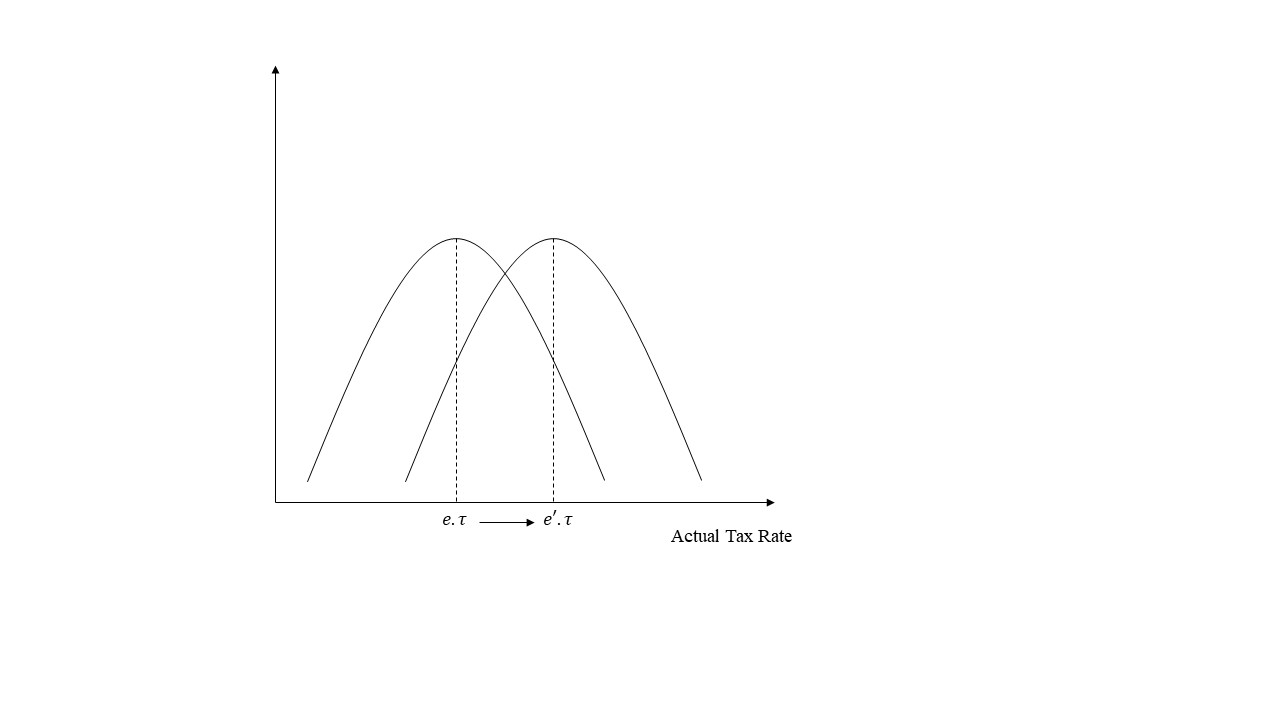
\includegraphics[scale=0.7]{Chapter-5/Figures/laffer.jpg}
%     \caption[Laffer Curve for Tax Collection Effort]{Laffer Curve for Tax Collection Effort
%         \texttt{} }
%     \label{laffer}
% \end{figure}

However, if both central and local governments prioritize welfare-related production expenditures beyond a certain threshold, the situation changes. In this case, increasing general transfers will encourage local governments to allocate more resources to the provision of welfare-related public goods. Consequently, increasing taxes will only exacerbate the crowding-out effect of high tax burdens on total production $F$. Therefore, increasing general transfers will instead prompt local governments to seek ways to alleviate tax burdens.

\subsection{The effect of categorical grants in productive area on tax collection effort}

Since $0<m<1$, whether equation \ref{mone} is positive or not is decided by denominator. Similarly, $1+\frac{\alpha \lambda_i(1-\sigma_i)}{1-\tau_i}$ also acts as a threshold. From the calculation, we have:

\begin{itemize}
    \item When $n_i+\lambda_i<1+\frac{\alpha \lambda_i(1-\sigma_i)}{1-\tau_i}$, $\frac{d \tau_i}{d m_i}>0$
    \item When $n_i+\lambda_i>1+\frac{\alpha \lambda_i(1-\sigma_i)}{1-\tau_i}$,$\frac{d \tau_i}{d m_i}<0$
\end{itemize}

When both national and subnational governments care less about welfare oriented spending, more categorical transfer on productive public goods would stimulate a higher tax collection effort, vice versa.

In the realm of categorical transfers, the effect of increasing the subsidy ratio for productive transfers by the central government on local tax efforts is entirely consistent with the increase in general transfers. This is not surprising, as even without restrictions on the usage domain of general transfers when both local and central governments prioritize productive public goods over welfare-related ones, local governments will still allocate more revenue to productive public goods. This parallels the effect of the central government stipulating a high matching ratio $m$ to encourage local governments to invest more in productive areas.

When both national and subnational governments care about the welfare oriented public goods such that $n+\lambda_i$ surpass the threshold, the greater matching ratio on productive public goods would not stimulate subnational government to invest more on productive spending. On the contrary, the relief on the productive investment would lead to lower revenue gap thus lower the tax collection effort.

\subsection{The effect of categorical grants in welfare area on tax collection effort}
The calculation and the expression of $\frac{\partial e_{i,t}}{\partial n}$ is complicated. I got the expression through Mathematica, the result is shown in figure \ref{enenen}.
% \begin{figure}[H]
%     \centering
%     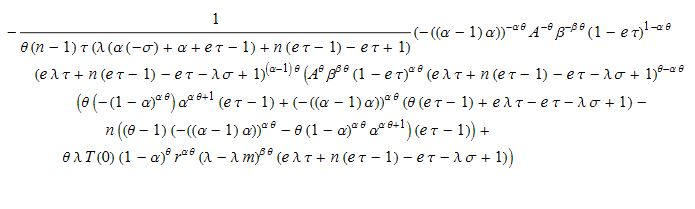
\includegraphics[scale=0.8]{Chapter-5/Figures/calculation effortttt.JPG}
%     \caption[Expression of $\frac{\partial e_{i,t}}{\partial n}$]{Expression of $\frac{\partial e_{i,t}}{\partial n}$
%         \texttt{} }
%     \label{enenen}
% \end{figure}

This expression is very complicated and hard to distinguish whether it's positive or negative, which means the effect of matching ratio of welfare-oriented public spending is ambiguous. We hypothesize that when the national government increases categorical transfers for welfare, it simultaneously incentivizes local governments to further increase the utility derived from welfare expenditures, thereby encouraging higher taxation. However, the role of taxation in economic growth is uncertain. Subnational government may want to decrease the tax collection revenue to boost the economic growth, since the investment in welfare is guaranteed by the subsidy. Therefore, the impact of increased welfare transfers on taxation incentives is uncertain.

For the following of this paper, I'll design an empirical investigation to statistically test my theoretical conjecture.

\section{Regression Model Design and Hypothesis}

This section is to give some general explain of the regression setting, such as the included factors and the regression model. In addition, I give my hypothesis about some of the factors based on the theoretical conjecture I get from previous Ramsey model.

The regression is to distinguish the effect of different kinds of intergovernmental transfer on the tax collection effort. Therefore, the dependent variable of this regression is the tax collection effort, which has been corrected using the Kalman filter algorithm. The specific algorithmic process will be detailed in subsequent sections. The independent variables consist of the ratio of general-purpose transfer payments to specific-purpose transfer payments. Our interest lies in exploring the impact of the growth or reduction of these ratio on tax collection efforts.

Based on our discussion of the theoretical model, there exists a "threshold effect" in the impact of general-purpose and specific-purpose transfer payments on tax collection efforts. The degree of emphasis placed by the federal and state governments on welfare-related public expenditures, represented as $n_i+\lambda_i$ plays a pivotal role in serving as such a threshold. Based on this theoretical inference, a moderating effect model would be particularly helpful in addressing our inquiry. Specifically, it would investigate how the effects of general-purpose and specific-purpose transfer payments on tax collection efforts are moderated by the degree of emphasis placed by the federal and state governments on welfare-related public expenditures.

\section{Variables and Sample}

This subsection is constructed to explain the meaning of the variables and how it's measured. The most important part is to explain the construction of moderating variables and how the dependent variable---tax collection effort is captures.

\subsection{Construction of moderating variables}
The moderating effect in this study exists between two pairs of variables: the variable $Ratio\_gen$, reflecting general-purpose transfer payments, and the variable $w_preference$ representing the degree of emphasis placed by the federal and local governments on welfare expenditures, respectively. Additionally, the moderating effect exists between the variable "transfer payments with purpose constraints" $Ratio\_cons$ and $w_preference$ Therefore, my regression model comprises two regression equations.

\begin{equation}
    TE_{i,t}=a+ \beta_1 Ratio\_gen_{i,t}+\beta_2 w\_preference_{i,t}+\beta_3(Ratio\_gen_{i,t}\cdot w\_preference_{i,t}) +\alpha_i CV_{i,t} \label{reg1}
\end{equation}

\begin{equation}
    TE_{i,t}=a+ \beta_4 Ratio\_cons_{i,t}+\beta_2 w\_preference_{i,t}+\beta_5(Ratio\_cons_{i,t}\cdot w\_preference_{i,t}) +\alpha_i CV_{i,t} \label{reg2}
\end{equation}

where CV means a set of control variables including ratio of different industrial sectors in the whole economy, such as agriculture, manufacturing, finance and insurance, trade and real estate and some factors reflecting economic condition such as gdp per capita, per capita expenditure, median household income and unemployment rate.


The construction of interacting variables is in regression \ref{reg1} and \ref{reg2} needs the representing of the general grants ratio $Ratio\_gen_{i,t}$, matching ratio on productive spending $Ratio\_cons_{i,t}$, and both level of governments' preference on welfare spending $w\_preference_{i,t}$.

From \textit{State Expenditure Annual Report} published by different state governments, I can classify federal and state governments' spending purpose into spending on productive and welfare oriented area. In addition, I can tell the source of the revenue by distinguishing if the grants is offered by federal or state governments. According to former investigation related to the classification of welfare spending and productive spending \parencite{AnpingZhao2012welfareexpenditure,lindbeck1988welfare,wlezien2021trends,stichnoth2013ethnic,schneider2005elite}, I group the spending on education, assistance on needy, cash assistance, medicaid, corrections as welfare spending and spending on transportation, housing and environment as productive expenditure\footnote{The abbreviation for welfare expenditure is marked as "W" in table \ref{expenditure} and productive expenditure is marked as "P". }.As also shown in table \ref{expenditure}, I can calculate whether the grants come from federal or states. Therefore I have the ratio of welfare expenditure of state and national government to represent the preference on welfare spending $w\_preferernce$.

White house Office of Management and Budget supplied publish federal's total outlay every year, in which we can find the proxy of general grants amounts  under "Federal funds" account and grants with constraint amounts under "Trust funds". The general grants amounts is clearly defined, while the ratio of productive grants and welfare grants need to be distinguished manually.

Every state in America is included in my sample and the time span last from 2000 to 2019, unless some specific data is missed.


% \begin{table}[htbp]
%     \centering
%     \caption{State Expenditure Purpose and Revenue Source}
%     \begin{tabular}{|l|c|c|c|c|r|}
%         \toprule
%                                                                                                 & \multicolumn{1}{p{4.355em}|}{General funds} & \multicolumn{1}{p{4.07em}|}{Federal funds} & \multicolumn{1}{p{5em}|}{Other State funds} & \multicolumn{1}{p{4.145em}|}{Bond funds} & \multicolumn{1}{p{6.785em}|}{\textit{\textbf{Expenditure Purposes}}} \\
%         \midrule
%         \multicolumn{1}{|p{9.93em}|}{Elementary \& Secondary Education }                        &                                             &                                            &                                             &                                          & \multicolumn{1}{c|}{\textbf{W}}                                      \\
%         \cmidrule{2-6}    \multicolumn{1}{|p{9.93em}|}{Higher Education }                       &                                             &                                            &                                             &                                          & \multicolumn{1}{c|}{\textbf{W}}                                      \\
%         \cmidrule{2-6}    \multicolumn{1}{|p{9.93em}|}{Temporary Assistance for Needy Families} &                                             &                                            &                                             &                                          & \multicolumn{1}{c|}{\textbf{W}}                                      \\
%         \cmidrule{2-6}    \multicolumn{1}{|p{9.93em}|}{Other Cash Assistance}                   &                                             &                                            &                                             &                                          & \multicolumn{1}{c|}{\textbf{W}}                                      \\
%         \cmidrule{2-6}    \multicolumn{1}{|p{9.93em}|}{Medicaid Total Funds}                    &                                             &                                            &                                             &                                          & \multicolumn{1}{c|}{\textbf{W}}                                      \\
%         \cmidrule{2-6}    \multicolumn{1}{|p{9.93em}|}{Corrections }                            &                                             &                                            &                                             &                                          & \multicolumn{1}{c|}{\textbf{W}}                                      \\
%         \cmidrule{2-6}    \multicolumn{1}{|p{9.93em}|}{Transportation }                         &                                             &                                            &                                             &                                          & \multicolumn{1}{c|}{\textbf{P}}                                      \\
%         \cmidrule{2-6}    \multicolumn{1}{|p{9.93em}|}{Housing Capital }                        &                                             &                                            &                                             &                                          & \multicolumn{1}{c|}{\textbf{P}}                                      \\
%         \cmidrule{2-6}    \multicolumn{1}{|p{9.93em}|}{Enviromental Capital }                   &                                             &                                            &                                             &                                          & \multicolumn{1}{c|}{\textbf{P}}                                      \\
%         \midrule
%         \textit{\textbf{Revenue Source}}                                                        & \textbf{State}                              & \textbf{Federal}                           & \textbf{State}                              & \textbf{---------}                       &                                                                      \\
%         \bottomrule
%     \end{tabular}%
%     \label{expenditure}%
% \end{table}%


The explain of the moderating effects coefficients are different compared to the normal regression. For example, in equation \ref{reg1}, $\beta_1$ is not the effect of general transfer on tax collection effort. To investigate the effect of general transfer ratio on dependent variable, I need to calculate $\frac{\partial TE_{i,t}}{\partial Ratio\_gen_{i,t}}$, thus I have:

$$\frac{\partial TE_{i,t}}{\partial Ratio\_gen_{i,t}}=\beta_1+\beta_3 \cdot w\_preference_{i,t} $$

Therefore, $\beta_1$ is not the effect of general transfer on the tax collection effect, rather, it means the effect of general transfer when $w\_preferernce_{i,t}=0$. As $w\_preferernce_{i,t}$ gets greater, we can tell the effect of general transfer on tax effort by analyzing $\beta_1+\beta_3$. This feature fits our previous theoretical conjecture perfectly since the preference on welfare public spending plays an threshold effect. We can better investigate this threshold effect through the moderating effect regression model. Based on the explain of this moderating effect regression and previous theoretical conjecture, I generated the first hypothesis.
\begin{itemize}
    \item \textbf{Hypothesis 1: Tax effort gets higher as general transfer ratio gets higher when both federal and state governments make light of welfare-oriented public spending. }
\end{itemize}

This hypotheses comes from the theoretical conjecture of the general transfer ratio. In the regression, my expectation is that $\beta_1$ is a significant positive value while $\beta_3$ is a significant negative value. In that way, the effect of general transfer ratio on tax collection effort is negative when $w_preference$ doesn't exceed the threshold. Once the $w_preference$ pass the specific threshold value, the increase of general transfer discourage the tax collection effort.

Similarly, I can have the hypotheses about the effect of productive categorical transfer increase on tax collection effort.

\begin{itemize}
    \item \textbf{Hypothesis 2: Tax effort gets higher as productive categorical transfer ratio gets higher when both federal and state governments make light of welfare-oriented public spending. }
\end{itemize}

The effect of productive categorical transfer follows same logic with the general transfers. Whether the increase of productive categorical transfer stimulates or suppress tax collection effort depends on if federal and state governments' preference on welfare spending surpass a specific threshold. Therefore I'm expecting a significant positive $\beta_4$ and negative $\beta_5$. When $w_preference$ gets greater, the effect of productive categorical transfer became negative.



\subsection{Measure of tax collection effort}

In terms of the dependent variable, tax collection effort, two methods are commonly employed: the average tax ratio method and the potential tax revenue method\parencite*{tait1978two,tanzi1981taxation,tanzi1983quantitative}. The former entails substituting the unobservable variable of tax collection with a proximate and measurable variable. Conversely, the latter method involves comparing the actual tax burden to the predicted tax burden using regression analysis, which is also called as "tax handle" method. According to \textcite{bahl1971regression}, an index of 1 means the tax effort is at the “expected” level, given the structural factors of that country. In other words, the country is using its taxable capacity at a level consistent with the average of the other countries in the sample \parencite{mertens2003measuring}.

However, \textcite{doi:10.1080/13504850500425345} has demonstrated that while the second method, compared to the first, provides relatively more reliable estimates of tax collection effort, both methods are inherently biased. In the same article, \textcite{doi:10.1080/13504850500425345} proposed a solution to this issue by using the Kalman filter to correct tax collection effort and proved its efficiency and unbiasedness in estimating tax collection effort. Therefore, this article also employs this approach to estimate tax collection effort for each state. Specifically, following Kim's methodology, the Kalman filter estimation of tax collection effort involves the following processes.

The state-space model is represented as:
\begin{equation}
    Y_t=\gamma X_t+\alpha A_t+\varepsilon_t \label{statespace1}
\end{equation}

\begin{equation}
    X_{t+1}=\beta X_t+\omega_{t+1}\label{statespace2}
\end{equation}

where $Y_t$ is the tax revenue at time $t$, $X_t$ is tax effort and $A_t$ is a vector of other factors affecting tax revenue except for tax effort. The error terms $\varepsilon_t$ and $\omega_{t}$ are both serially uncorrelated with a mean of zero and a covariance matrix $h_t$ and $q_t$ respectively. Therefore we have:

\begin{equation}
    (\begin{array}{l}\varepsilon_t \\ \omega_t\end{array}) \sim N\left(\left(\begin{array}{l}0 \\ 0\end{array}\right) ,\left(\begin{array}{ll}h_t & 0 \\ 0 & q_t\end{array}\right)\right) \label{ssvar}
\end{equation}

$X_t$ has a known mean $a_0 $and a variance $b_0$. Therefore, if the variances of the error terms and the initial values of revenue effort and its variance are known, tax revenue effort can be derived with the following Kalman filter equations \parencite{doi:10.1080/13504850500425345}:

\begin{equation}
    \hat{X}_{t+1,t}=\tau \hat{X}_{t,t}\label{k1}
\end{equation}

\begin{equation}
    P_{t+1,t}=\tau^2 P_{t,t}+q^2
\end{equation}

\begin{equation}
    B_{t+1,t}=\alpha^2 P_{t+1,t}+h^2
\end{equation}

\begin{equation}
    \hat{\epsilon}_{t+1,t}=Y_{t+1}-\alpha \hat{X}_{t+1,t}-\beta A_{t+1}
\end{equation}

\begin{equation}
    K_{t+1}=P_{t+1,t}\alpha B^{-1}_{t+1,t}
\end{equation}

\begin{equation}
    \hat{X}_{t+1,t+1}=\hat{X}_{t+1,t}+K_{t+1}\hat{\epsilon}_{t+1,t}
\end{equation}

\begin{equation}
    P_{t+1,t+1}=(1-K_{t+1}\alpha)P_{t+1,t}\label{k7}
\end{equation}

From equation \ref{k1} to equation \ref{k7}, I can get a kalman filter processed series data \{$X_{t,t}$\} of each state i. Now I need to specify the state-space model formed up by measurement equation, which is equation \ref{statespace1} and transition equation, which is equation \ref{statespace2}.

Equation \ref{statespace1} is the commonly used "tax handle" regression. I focus on the tax collection effort of states governments, thus the commonly used tax handle should includes the factors that reflect the economic structure. Based on the North American Industry Classification System (NAICS), I categorized all industries into 11 major groups: Agriculture; Mining; Manufacturing; Wholesale trade and retail trade; Transportation and warehousing; Information; Finance and insurance; Real estate, rental, and leasing; Health care and social assistance; Professional, scientific, educational, and technical services. I'll calculate the ratio of each industries compared to state GDP and make it as tax handles. Besides, the commonly used control variables to predict the tax revenue includes GDP per capita, median household income and unemployment rate. Therefore the variables included in $A_t$ can be listed as table \ref{handlevariables}.
% Table generated by Excel2LaTeX from sheet 'xtregionolsss0212'
% \begin{table}[htbp]
%     \centering
%     \caption{Tax handle variables to predict the tax revenue}
%     \begin{tabular}{cl}
%         \toprule
%         Abbreviation & Meaning                                                       \\
%         \midrule
%         agrr         & Ratio of agriculture to gdp                                   \\
%         minr         & Ratio of mining to gdp                                        \\
%         manr         & Ratio of manufacturing to gdp                                 \\
%         tandwr       & Ratio of transportation and warehouse to gdp                  \\
%         infr         & Ratio of information to gdp                                   \\
%         fandir       & Ratio of finance and insurance to gdp                         \\
%         rer          & Ratio of real estate to gdp                                   \\
%         hsr          & Ratio of health care and social assistance to gdp             \\
%         piepcm       & per capital income spend on expenditure                       \\
%         trader       & Ratio of trade to gdp                                         \\
%         pster        & Professional, scientific, educational, and technical services \\
%         mehim        & Median household income                                       \\
%         unemployrate & unemployment rate                                             \\
%         gdp          & GDP per capita                                                \\
%         \bottomrule
%     \end{tabular}%
%     \label{handlevariables}%
% \end{table}%

Given the diverse economic structures across different regions in the United States, industries serving as tax bases vary. Recognizing the variation in tax bases created by different economic structures in various regions, I segmented the data by region to conduct fixed-effects regressions based on the U.S. Department of Commerce Bureau of Economic Analysis' classification of regions , aiming to maximize the adjusted R-squared and enhance predictive accuracy. Those 8 segments are: Far West, Great Lakes, Mideast, New England,	Plains,	Rocky Mountain,	Southeast, Southwest.

The DF test result, shown in table \ref{DFtest} for each variable within each region shows that some time series data are not stationary, which contradicts with the assumption of equation \ref{ssvar}. Therefore before the tax handle regression, I conduct the 1 st order difference for the variables that do not pass the DF test and make sure all variables of states $i$ are stationary before conducting the tax handle regression \footnote{Table \ref{DFtest} only shows part of the DF test results. For full results, please visit the appendix part}.

% Table generated by Excel2LaTeX from sheet 'processedDFTEST0212'
% \begin{table}
%     \centering
%     \caption{DF test results for variables in state of America}
%     \resizebox{17cm}{11cm}{
%         \begin{tabular}{llrrrrrrrrrrrrrrr}
%             \toprule
%             geoname     & level\_1      & \multicolumn{1}{l}{taxrevenueratio} & \multicolumn{1}{l}{agrr} & \multicolumn{1}{l}{minr} & \multicolumn{1}{l}{manr} & \multicolumn{1}{l}{tandwr} & \multicolumn{1}{l}{infr} & \multicolumn{1}{l}{fandir} & \multicolumn{1}{l}{rer} & \multicolumn{1}{l}{hsr} & \multicolumn{1}{l}{piepcm} & \multicolumn{1}{l}{trader} & \multicolumn{1}{l}{pster} & \multicolumn{1}{l}{mehim} & \multicolumn{1}{l}{unemployrate} & \multicolumn{1}{l}{gdppercapita} \\
%             \midrule
%             Alabama     & ADF Statistic & -2.9584957                          & -4.0738483               & -2.1262916               & -3.7780187               & -2.3795241                 & -4.5285992               & -2.8465617                 & -3.3691314              & -6.6545878              & -2.3099791                 & -0.354905                  & -4.7383288                & -5.2118955                & -2.5388273                       & -2.4977533                       \\
%             Alabama     & P-value       & 0.1440567                           & 0.0068865                & 0.531346                 & 0.0177068                & 0.3905597                  & 0.0013549                & 0.1803687                  & 0.0556509               & 8.41E-08                & 0.4284382                  & 0.9881567                  & 0.0005996                 & 8.32E-05                  & 0.3088295                        & 0.3290865                        \\
%             Alaska      & ADF Statistic & -2.0826184                          & -3.1155341               & -3.7940843               & -3.3981553               & -6.4811537                 & -2.6940316               & -4.9448154                 & -4.5470878              & -5.6889734              & -3.1354863                 & -7.3714471                 & -3.0392903                & -1.7603157                & -2.7177455                       & -2.7181459                       \\
%             Alaska      & P-value       & 0.5558153                           & 0.1025832                & 0.0168625                & 0.0516349                & 2.03E-07                   & 0.238569                 & 0.000259                   & 0.0012629               & 9.64E-06                & 0.0980398                  & 2.01E-09                   & 0.1214254                 & 0.7235718                 & 0.2287886                        & 0.2286257                        \\
%             Arizona     & ADF Statistic & -3.8693215                          & -4.6322823               & -1.7101206               & -0.3743152               & -7.5316714                 & -4.4778336               & -4.1707467                 & -5.3301527              & -2.5375428              & -2.0054682                 & -2.3710659                 & -3.7761038                & -6.1423639                & -1.9470851                       & -2.5295149                       \\
%             Arizona     & P-value       & 0.0133634                           & 0.0009099                & 0.7464038                & 0.9876256                & 8.62E-10                   & 0.0016406                & 0.0049542                  & 4.95E-05                & 0.3094533               & 0.5984518                  & 0.3951099                  & 0.0178099                 & 1.10E-06                  & 0.6299357                        & 0.3133664                        \\
%             Arkansas    & ADF Statistic & -3.8144652                          & -3.2574705               & -3.3138418               & -3.2526213               & -2.6120583                 & -3.0102396               & -5.2714893                 & -1.9617547              & -3.8665392              & -2.8672628                 & 0.7610834                  & -3.8232961                & -7.2296709                & -1.8315081                       & -2.9306735                       \\
%             Arkansas    & P-value       & 0.0158426                           & 0.0735461                & 0.0640084                & 0.0744169                & 0.2743734                  & 0.1292407                & 6.41E-05                   & 0.6221029               & 0.0134803               & 0.1733367                  & 1                          & 0.0154179                 & 4.25E-09                  & 0.6893708                        & 0.1525052                        \\
%             California  & ADF Statistic & -3.3335918                          & 0.7247841                & -5.2060476               & -2.2999803               & -3.9951928                 & -1.4944674               & -3.301189                  & -5.0087446              & -5.1396849              & -2.3659968                 & -2.8818869                 & -3.6344666                & -2.2391546                & -2.2533527                       & -2.8013711                       \\
%             California  & P-value       & 0.0609133                           & 1                        & 8.53E-05                 & 0.4339608                & 0.008933                   & 0.8310186                & 0.0660573                  & 0.0001983               & 0.0001137               & 0.3978451                  & 0.1684937                  & 0.027052                  & 0.4678524                 & 0.4599033                        & 0.1964413                        \\
%             Colorado    & ADF Statistic & -7.6191717                          & -3.3285227               & -0.8284793               & -2.0928674               & -2.7511687                 & -2.1354386               & -4.6806141                 & -2.6886979              & -4.714105               & -2.3839804                 & -1.2484704                 & -3.8171345                & -4.353958                 & -2.0836961                       & -2.559226                        \\
%             Colorado    & P-value       & 5.42E-10                            & 0.0616959                & 0.9631981                & 0.5500885                & 0.2154567                  & 0.5262035                & 0.0007533                  & 0.2408052               & 0.0006601               & 0.3881694                  & 0.9000907                  & 0.0157131                 & 0.0025905                 & 0.5552137                        & 0.2990106                        \\
%             Connecticut & ADF Statistic & 0.105427                            & -5.614409                & -2.6514881               & -3.7322998               & -3.3657117                 & -2.1895655               & -3.9815021                 & -2.9085756              & -3.7505465              & -2.7743348                 & -2.5193086                 & -3.2045364                & -2.5030802                & -3.7037153                       & -4.7590079                       \\
%             Connecticut & P-value       & 0.9951566                           & 1.36E-05                 & 0.2567715                & 0.0203164                & 0.0561405                  & 0.495725                 & 0.0093407                  & 0.1594584               & 0.0192371               & 0.2065306                  & 0.3183769                  & 0.0835016                 & 0.326424                  & 0.0221138                        & 0.0005522                        \\
%             Delaware    & ADF Statistic & -3.1393466                          & -3.3145667               & -4.9336125               & -3.2188079               & -0.7223429                 & -2.303585                & -0.6156446                 & -3.3056062              & -4.247519               & -2.7340805                 & -3.7018074                 & -5.8610316                & -4.7405574                & -3.2199067                       & -10.574259                       \\
%             Delaware    & P-value       & 0.0971789                           & 0.0638926                & 0.0002713                & 0.0807187                & 0.9716374                  & 0.431968                 & 0.9781385                  & 0.0653361               & 0.0037908               & 0.2222062                  & 0.0222385                  & 4.28E-06                  & 0.0005943                 & 0.0805075                        & 1.51E-16                         \\
%             Florida     & ADF Statistic & -4.8669747                          & -2.7072056               & -4.2669358               & -5.5067657               & -2.6650288                 & -0.4769127               & -1.9741621                 & -3.3385817              & -3.0333683              & -3.0453498                 & -2.4700988                 & -5.2922004                & -2.136408                 & -2.542309                        & -2.5571086                       \\
%             Florida     & P-value       & 0.0003569                           & 0.2331029                & 0.0035394                & 2.23E-05                 & 0.2508878                  & 0.9843121                & 0.6154352                  & 0.0601509               & 0.1229896               & 0.1198402                  & 0.3430694                  & 5.85E-05                  & 0.5256582                 & 0.307142                         & 0.3000221                        \\
%             Georgia     & ADF Statistic & -1.3862558                          & -3.9642423               & -1.5576629               & -3.974274                & -1.4218962                 & -1.0532807               & -2.1118196                 & -3.6462642              & -4.011087               & -2.0314994                 & -3.7304951                 & -2.7878658                & -2.8849757                & -2.4816295                       & -0.3230385                       \\
%             Georgia     & P-value       & 0.8649024                           & 0.0098784                & 0.8085722                & 0.0095626                & 0.8543696                  & 0.9365038                & 0.5394719                  & 0.0261488               & 0.0084799               & 0.5841755                  & 0.020426                   & 0.2014369                 & 0.1674839                 & 0.3372069                        & 0.9889707                        \\
%             Hawaii      & ADF Statistic & -3.2823748                          & -3.4492431               & -2.0175917               & -0.9805192               & -4.2261142                 & -3.5835385               & -4.2564581                 & 0.1945429               & -2.9148399              & -1.8186507                 & -3.3759258                 & -1.5834406                & -0.9607372                & -3.2727731                       & -2.0802754                       \\
%             Hawaii      & P-value       & 0.0692012                           & 0.045148                 & 0.591819                 & 0.9466804                & 0.0040869                  & 0.0312658                & 0.0036731                  & 0.9957462               & 0.1574654               & 0.6956964                  & 0.0546885                  & 0.79885                   & 0.9491729                 & 0.0708514                        & 0.5571229                        \\
%             Idaho       & ADF Statistic & -4.272711                           & -3.4487125               & -1.8967678               & -3.0275766               & -3.109667                  & -2.7050241               & 0.1819603                  & -2.7692856              & -4.7744075              & -2.9283954                 & 0.1210051                  & -3.6201161                & -11.799223                & -2.9882011                       & -3.5448589                       \\
%             Idaho       & P-value       & 0.0034676                           & 0.0452117                & 0.6563424                & 0.1245337                & 0.1039492                  & 0.2340024                & 0.9956721                  & 0.2084541               & 0.0005192               & 0.153212                   & 0.995271                   & 0.0281867                 & 8.23E-19                  & 0.1354096                        & 0.0348303                        \\
%             Illinois    & ADF Statistic & 2.2055768                           & -4.5868314               & -2.9059329               & -2.9685475               & -4.9050819                 & -4.0010139               & -3.1577302                 & -4.0337167              & -3.3368733              & -2.8416788                 & -2.1622079                 & -4.5311699                & -4.8661301                & -2.6609907                       & -3.1650605                       \\
%             Illinois    & P-value       & 1                                   & 0.0010847                & 0.1603045                & 0.1410877                & 0.0003053                  & 0.0087646                & 0.0931582                  & 0.0078705               & 0.0604111               & 0.1820576                  & 0.5111346                  & 0.0013417                 & 0.0003581                 & 0.2526337                        & 0.0915913                        \\
%             Indiana     & ADF Statistic & -5.1574461                          & -5.7155784               & -2.1507255               & -6.4777512               & -3.06508                   & -5.2218945               & -7.0097004                 & -6.1401189              & -7.8039373              & -2.436235                  & -2.3102721                 & -3.0872072                & -0.7023714                & -2.9533594                       & -3.6019904                       \\
%             Indiana     & P-value       & 0.0001053                           & 8.51E-06                 & 0.5176008                & 2.06E-07                 & 0.1147847                  & 7.96E-05                 & 1.34E-08                   & 1.11E-06                & 2.03E-10                & 0.3605396                  & 0.4282766                  & 0.1093063                 & 0.9729916                 & 0.1455909                        & 0.0296783                        \\
%             Iowa        & ADF Statistic & -6.0901826                          & -4.3927572               & -2.4832443               & -7.0679353               & -2.6322937                 & -1.9978792               & -5.5354435                 & -3.1579108              & -4.6701772              & -3.2590251                 & -3.2725052                 & -2.7406905                & -6.0708915                & -2.9988559                       & -4.9323914                       \\
%             Iowa        & P-value       & 1.42E-06                            & 0.0022487                & 0.3363895                & 9.91E-09                 & 0.2652539                  & 0.6025886                & 1.96E-05                   & 0.0931194               & 0.0007848               & 0.0732687                  & 0.0708978                  & 0.2195788                 & 1.56E-06                  & 0.1324011                        & 0.0002727                        \\
%             Kansas      & ADF Statistic & -2.5665144                          & -3.1387984               & -1.2040844               & 0.61863                  & -2.9471436                 & -4.2537381               & -2.7062164                 & -2.4390351              & -0.5887284              & -3.0432453                 & -2.7899665                 & -4.5161056                & -3.8964404                & -2.7820881                       & -4.1499461                       \\
%             Kansas      & P-value       & 0.2955427                           & 0.0973008                & 0.9096626                & 0.9970018                & 0.1474629                  & 0.0037085                & 0.2335105                  & 0.3590813               & 0.9795168               & 0.120389                   & 0.2006541                  & 0.0014205                 & 0.0122702                 & 0.2036011                        & 0.0053214                        \\
%             Kentucky    & ADF Statistic & -3.7910525                          & -2.556417                & -4.9316617               & -2.4623514               & -3.140775                  & -2.6790055               & -2.6041511                 & -3.3248058              & -0.7279646              & -2.8402648                 & -2.0194022                 & -0.6672932                & -4.0015556                & -2.519608                        & -4.1190233                       \\
%             Kentucky    & P-value       & 0.0170191                           & 0.3003528                & 0.0002735                & 0.3470336                & 0.0968618                  & 0.2449027                & 0.2779856                  & 0.0622749               & 0.9712438               & 0.1825489                  & 0.590826                   & 0.9752111                 & 0.008749                  & 0.3182293                        & 0.0059134                        \\
%             Louisiana   & ADF Statistic & -3.4668779                          & -7.3993455               & -5.0297387               & -3.123526                & -2.0422269                 & 0.5809776                & -2.7602631                 & -3.158981               & -4.0690225              & -2.6377381                 & -2.5084001                 & -1.8975846                & -3.0377071                & -1.4466776                       & -3.5362443                       \\
%             Louisiana   & P-value       & 0.0430729                           & 1.74E-09                 & 0.0001816                & 0.1007445                & 0.5782566                  & 0.9969685                & 0.2119217                  & 0.0928894               & 0.0069986               & 0.2628312                  & 0.3237753                  & 0.6559199                 & 0.1218422                 & 0.8466851                        & 0.0356696                        \\
%             \bottomrule
%         \end{tabular}%
%         \label{DFtest}}%
% \end{table}%



Given that the primary objective of this regression equation is prediction, multicollinearity is not a significant concern. The tax handle regression results can be listed as table \ref{taxhandleregressionresult}. In this table, we can tell clearly that the significant industries, which is tax handles that determinant the tax revenue of states, are different. For example, the manufacturing industry is important for states in Plains area, while it's not significant for other areas such as states in far west, great lakes, mideast and new england. This also reflects the significance to predict the revenue and conduct the tax handle regression by region.

The tax handle regression in different regions are listed in Table \ref{taxhandleregressionresult}. After removing the insignificant factors, I get the predicted tax revenue ratio based on the significant tax handles. For example, for states in far west area, the predict formula is listed as:

\begin{equation}
    Tax\_revenue\_predict= tandw* 1.674 + fandi * 1.133 -3.223* hs  + trade * 0.818 + gdppercapita * 0.029 \label{taxhandlefarwest}
\end{equation}



% \begin{table}
%     \centering
%     \caption{Tax handle regression results for regions in America}
%     \resizebox{\textwidth}{8cm}{
%         \begin{tabular}{ccccccccc}
%             \toprule
%                                         & Far West  & Great Lakes & Mideast    & New England & Plains     & Rocky Mountain & Southeast  & Southwest   \\
%             \midrule
%             agrr                        & 0.314     & 0.391       & 0.478      & 1.169       & 0.038      & -0.115         & 0.0381     & 0.69        \\
%                                         & -0.27     & -1.06       & -0.74      & -1.55       & -1.18      & (-0.44)        & -0.29      & -1.53       \\
%             minr                        & 0.185     & 0.031       & 0.653      & -0.248      & 0.156      & -0.0348        & 0.0343     & 0.0859      \\
%                                         & -1.87     & -0.08       & -1.91      & (-0.28)     & -0.87      & (-1.15)        & -0.48      & -1.24       \\
%             manr                        & -0.0354   & 0.0383      & -0.0819    & 0.0375      & -0.130**   & 0.0179         & 0.0746     & -0.0132     \\
%                                         & (-0.30)   & -0.77       & (-0.97)    & -0.74       & (-3.03)    & -0.16          & -1.04      & (-0.31)     \\
%             tandwr                      & 1.674***  & 1.493***    & 1.205***   & -1.131*     & -0.138     & 0.12           & 1.092***   & 0.17        \\
%                                         & -22.19    & -27.17      & -4.2       & (-2.29)     & (-0.89)    & -0.39          & -22.7      & -0.89       \\
%             infr                        & -0.16     & -0.28       & -0.0533    & -0.0324     & -0.0277    & 0.061          & -0.0518    & -0.362*     \\
%                                         & (-0.62)   & (-0.79)     & (-0.65)    & (-0.24)     & (-0.38)    & -0.24          & (-0.32)    & (-2.41)     \\
%             fandir                      & 1.133*    & -0.109      & -0.0168    & 0.0688      & 0.0799*    & -0.268         & -0.541***  & 0.0148      \\
%                                         & -2.76     & (-0.72)     & (-0.37)    & -1.65       & -2.78      & (-1.00)        & (-23.22)   & -0.08       \\
%             rer                         & -0.069    & 0.00559     & -0.120**   & 0.161*      & 0.189***   & -0.0876        & -0.0218    & 0.158***    \\
%                                         & (-0.43)   & -0.84       & (-2.94)    & -2.26       & -4.71      & (-1.24)        & (-0.57)    & -5.85       \\
%             hsr                         & -3.223**  & 0.262       & -0.0815    & 0.317**     & -0.0291    & 1.138*         & 0.756***   & -1.326*     \\
%                                         & (-3.17)   & -0.82       & (-1.19)    & -3.23       & (-0.09)    & -2.23          & -28.81     & (-2.19)     \\
%             piepcm                      & 0.017     & 0.022       & 0.00506*   & 0.00597     & 0.00863    & -0.00616       & 0.00248*   & 0.0329      \\
%                                         & -0.3      & -0.97       & -2.66      & -0.71       & -0.4       & (-1.46)        & -2.24      & -1.17       \\
%             trader                      & 0.818*    & 0.0534      & -0.155**   & -0.105      & 0.0846     & -0.203*        & -0.0765    & -0.209***   \\
%                                         & -2.63     & -0.29       & (-3.57)    & (-0.88)     & -0.46      & (-2.14)        & (-2.06)    & (-7.11)     \\
%             pster                       & -0.45     & 0.0163      & 0.0194     & 0.189       & 0.507      & -0.137         & 0.788***   & -0.146      \\
%                                         & (-1.02)   & -0.89       & -0.21      & -1.86       & -1.88      & (-0.43)        & -35.78     & (-0.59)     \\
%             mehim                       & -0.00209  & 0.000118    & -0.00259*  & 0.00166     & 0.00102    & 0.00367*       & -0.00033   & -0.00409*** \\
%                                         & (-0.90)   & -0.11       & (-2.28)    & -1.61       & -0.79      & -2.44          & (-2.03)    & (-6.63)     \\
%             unemployrate                & 0.00127   & 0.00147     & 0.00128*   & 0.000011    & 0.00227    & 0.00185        & 0.000567** & 0.00187*    \\
%                                         & -1.25     & -1.56       & -2.75      & -0.01       & -1.65      & -1.92          & -3.52      & -2.66       \\
%             gdppercapita                & 0.0295*** & -0.00041    & 0.00397*** & 0.000235    & 0.00632*** & 0.00113        & 0.000338   & -0.0353**   \\
%                                         & -5.38     & (-0.89)     & -4.2       & -0.32       & -7.52      & -0.22          & -1.25      & (-3.52)     \\
%             Constant                    & -0.00177  & -0.00194    & 0.0201*    & -0.0149*    & -0.00177   & 0.0147         & -1.5E-05   & 0.0247***   \\
%                                         & (-0.33)   & (-0.80)     & -2.72      & (-2.76)     & (-0.86)    & -0.64          & (-0.02)    & -5.27       \\
%             \midrule
%             Observations                & 98        & 93          & 87         & 86          & 117        & 79             & 210        & 68          \\
%             Adjusted R-sq               & 0.882     & 0.982       & 0.988      & 0.979       & 0.963      & 0.893          & 0.958      & 0.98        \\
%             \midrule
%             t statistics in parentheses &           &             &            &             &            &                &            &             \\
%             *p<0.05,**p<0.01,***p<0.001 &           &             &            &             &            &                &            &             \\
%             \bottomrule
%         \end{tabular}}%
%     \label{taxhandleregressionresult}%
% \end{table}%

After the tax handle regression, I get the predicted tax revenue ratio for different state. Then I can get the tax collection effort by calculating the predicted value with actual value $\frac{Tax\_revenue\_predict}{Tax\_revenue\_actual}$. Part of the descriptive results is shown in table \ref{taxeffortsum}. Therefore, I have the measurement equation ready among the space-state equations since I have $X_t$ in equation \ref{statespace1} known parameters. In addition, the B-W heteroskedasticity test confirms that regression of equation \ref{statespace1} follows the constant residuals, shown in table \ref{bwtest}

% \begin{table}[htbp]
%     \centering
%     \caption{B-W heteroskedasticity test result for measurement equation regression}
%     \begin{tabular}{llllll}
%         \toprule
%         \multicolumn{6}{c}{Breusch-Pagan / Cook-Weisberg test for heteroskedasticity } \\
%         \midrule
%         \multicolumn{6}{l}{         Ho: Constant variance}                             \\
%         \multicolumn{6}{l}{         Variables: residuals}                              \\
%         \multicolumn{6}{c}{}                                                           \\
%         \multicolumn{6}{l}{         chi2(1)      =     0.88}                           \\
%         \multicolumn{6}{l}{         Prob > chi2  =   0.3491}                           \\
%         \bottomrule
%     \end{tabular}%
%     \label{bwtest}%
% \end{table}%


For transition equations, I assume the transition process follows an AR(1) process and the coefficient of the autocorrelation is 1 since table \ref{taxeffortsum} shows most of the tax effort index lies in [0.7, 1.2] and the standard error is small\footnote{This assumption is not necessarily to be too precise.}.

So far I got the space-state equation prepared and the initial parameters for kalman filter process is known including $\gamma$, $\alpha$, $\alpha$, $X_{0,0}$, $P_{0,0}$. Therefore, through equation \ref{k1} to equation \ref{k7}, I have a new kalman algorithm adjusted series of tax collection effort $\{X_{t,t}\}$.


% \begin{table}[htbp]
%     \centering
%     \caption{Summary of the tax effort level in states(part)}
%     \begin{tabular}{cccccc}
%         \toprule
%                     &     & \multicolumn{4}{c}{Tax collection effort}                               \\
%         \midrule
%         State       & Obs & Mean                                      & Std.    & Min     & Max     \\
%         \midrule
%         Alabama     & 17  & 0.99108                                   & 0.10704 & 0.77345 & 1.12369 \\
%         Alaska      & 18  & 1.15363                                   & 0.63936 & -0.0749 & 2.9033  \\
%         Arizona     & 15  & 0.9645                                    & 0.10226 & 0.80104 & 1.19916 \\
%         Arkansas    & 15  & 0.97468                                   & 0.12192 & 0.85674 & 1.20869 \\
%         California  & 19  & 1.05056                                   & 0.16872 & 0.53894 & 1.23222 \\
%         Colorado    & 19  & 1.01097                                   & 0.10623 & 0.8695  & 1.26189 \\
%         Connecticut & 19  & 0.73208                                   & 0.08448 & 0.6359  & 0.90594 \\
%         Delaware    & 14  & 1.08929                                   & 0.09726 & 0.90916 & 1.2335  \\
%         Florida     & 19  & 1.09674                                   & 0.16283 & 0.87646 & 1.49477 \\
%         Georgia     & 19  & 0.99922                                   & 0.1371  & 0.74665 & 1.34715 \\
%         Hawaii      & 14  & 0.97187                                   & 0.15959 & 0.69107 & 1.18888 \\
%         Idaho       & 19  & 0.91308                                   & 0.11257 & 0.73638 & 1.18433 \\
%         Illinois    & 19  & 1.00037                                   & 0.1077  & 0.82428 & 1.26365 \\
%         Indiana     & 17  & 1.00917                                   & 0.07028 & 0.85208 & 1.13589 \\
%         Iowa        & 17  & 8.06824                                   & 1.30505 & 5.15989 & 9.82793 \\
%         Kansas      & 19  & 1.23506                                   & 0.18167 & 0.9192  & 1.70648 \\
%         Kentucky    & 19  & 0.9929                                    & 0.08475 & 0.87784 & 1.25705 \\
%         \bottomrule
%     \end{tabular}%
%     \label{taxeffortsum}%
% \end{table}%

After the estimation of tax collection effort, I can run regression \ref{reg1} and regression \ref{reg2}. The results can be listed as Table \ref{reg_igt_eff}

\section{Regression Results and Analysis}

The regression result is shown in table \ref{reg_igt_eff}. Both OLS regression and fixed regression, with state and time fixed, are adopted with different variables included. To control the heteroskedasticity problem, I included robust standard error in both regressions. The adjusted R-square and the significance of all models are acceptable, but I adopt the coefficients of fixed effect model as reference, in which state and time variable fixed.

The first hypotheses about the general transfer ratio is supported. From model 4, the coefficient of $generalratio$ is 17.64 and it's significant on 5\% confident level. The coefficient of the interaction variable $int_gen_pref$ is -23.64 and it's also statistically significant. This coefficients combination strongly supported our hypotheses about the effect of general grants on tax collection effort: when federal and state government care less about the welfare-oriented public spending, more general transfer lead to higher tax collection effort. For example, when both levels of governments do not care about welfare at all, which means $n+\lambda=0$, $\frac{\partial\ TE}{\partial generalratio}=\beta_1=17.64$. Once federal or state government attach importance to the welfare product, thus federal increase the matching ratio of welfare spending $n$ and state government get more utility for welfare spending, which makes $n+\lambda_i$ pass the threshold, the marginal effect of general transfer ratio on tax collection effort became negative. For example, when $n+\lambda=1$, $\frac{\partial TE}{\partial generalratio}=\beta_1+\beta_3=-6$.

The second hypothesis is not supported unfortunately. On the contrary, the coefficient of constraint ratio $\beta_4$ in model 3 equals to -14.38 and the coefficient of the interaction term $int_cons_pref$ equals to 19.25. This means that, though we do observe an threshold effect, the effect is not act similarly with general transfer, just the opposite, the marginal effect on the matching ratio on productive spending $m$ is positive when both levels of governments neglect the welfare spending, and such marginal effect turns to negative when $n+\lambda$ exceeds the threshold.

The moderating effect of the two regression models are represented in figure \ref{int_gen_W} and \ref{int_cons_W}.

% \begin{figure}[H]
%     \centering
%     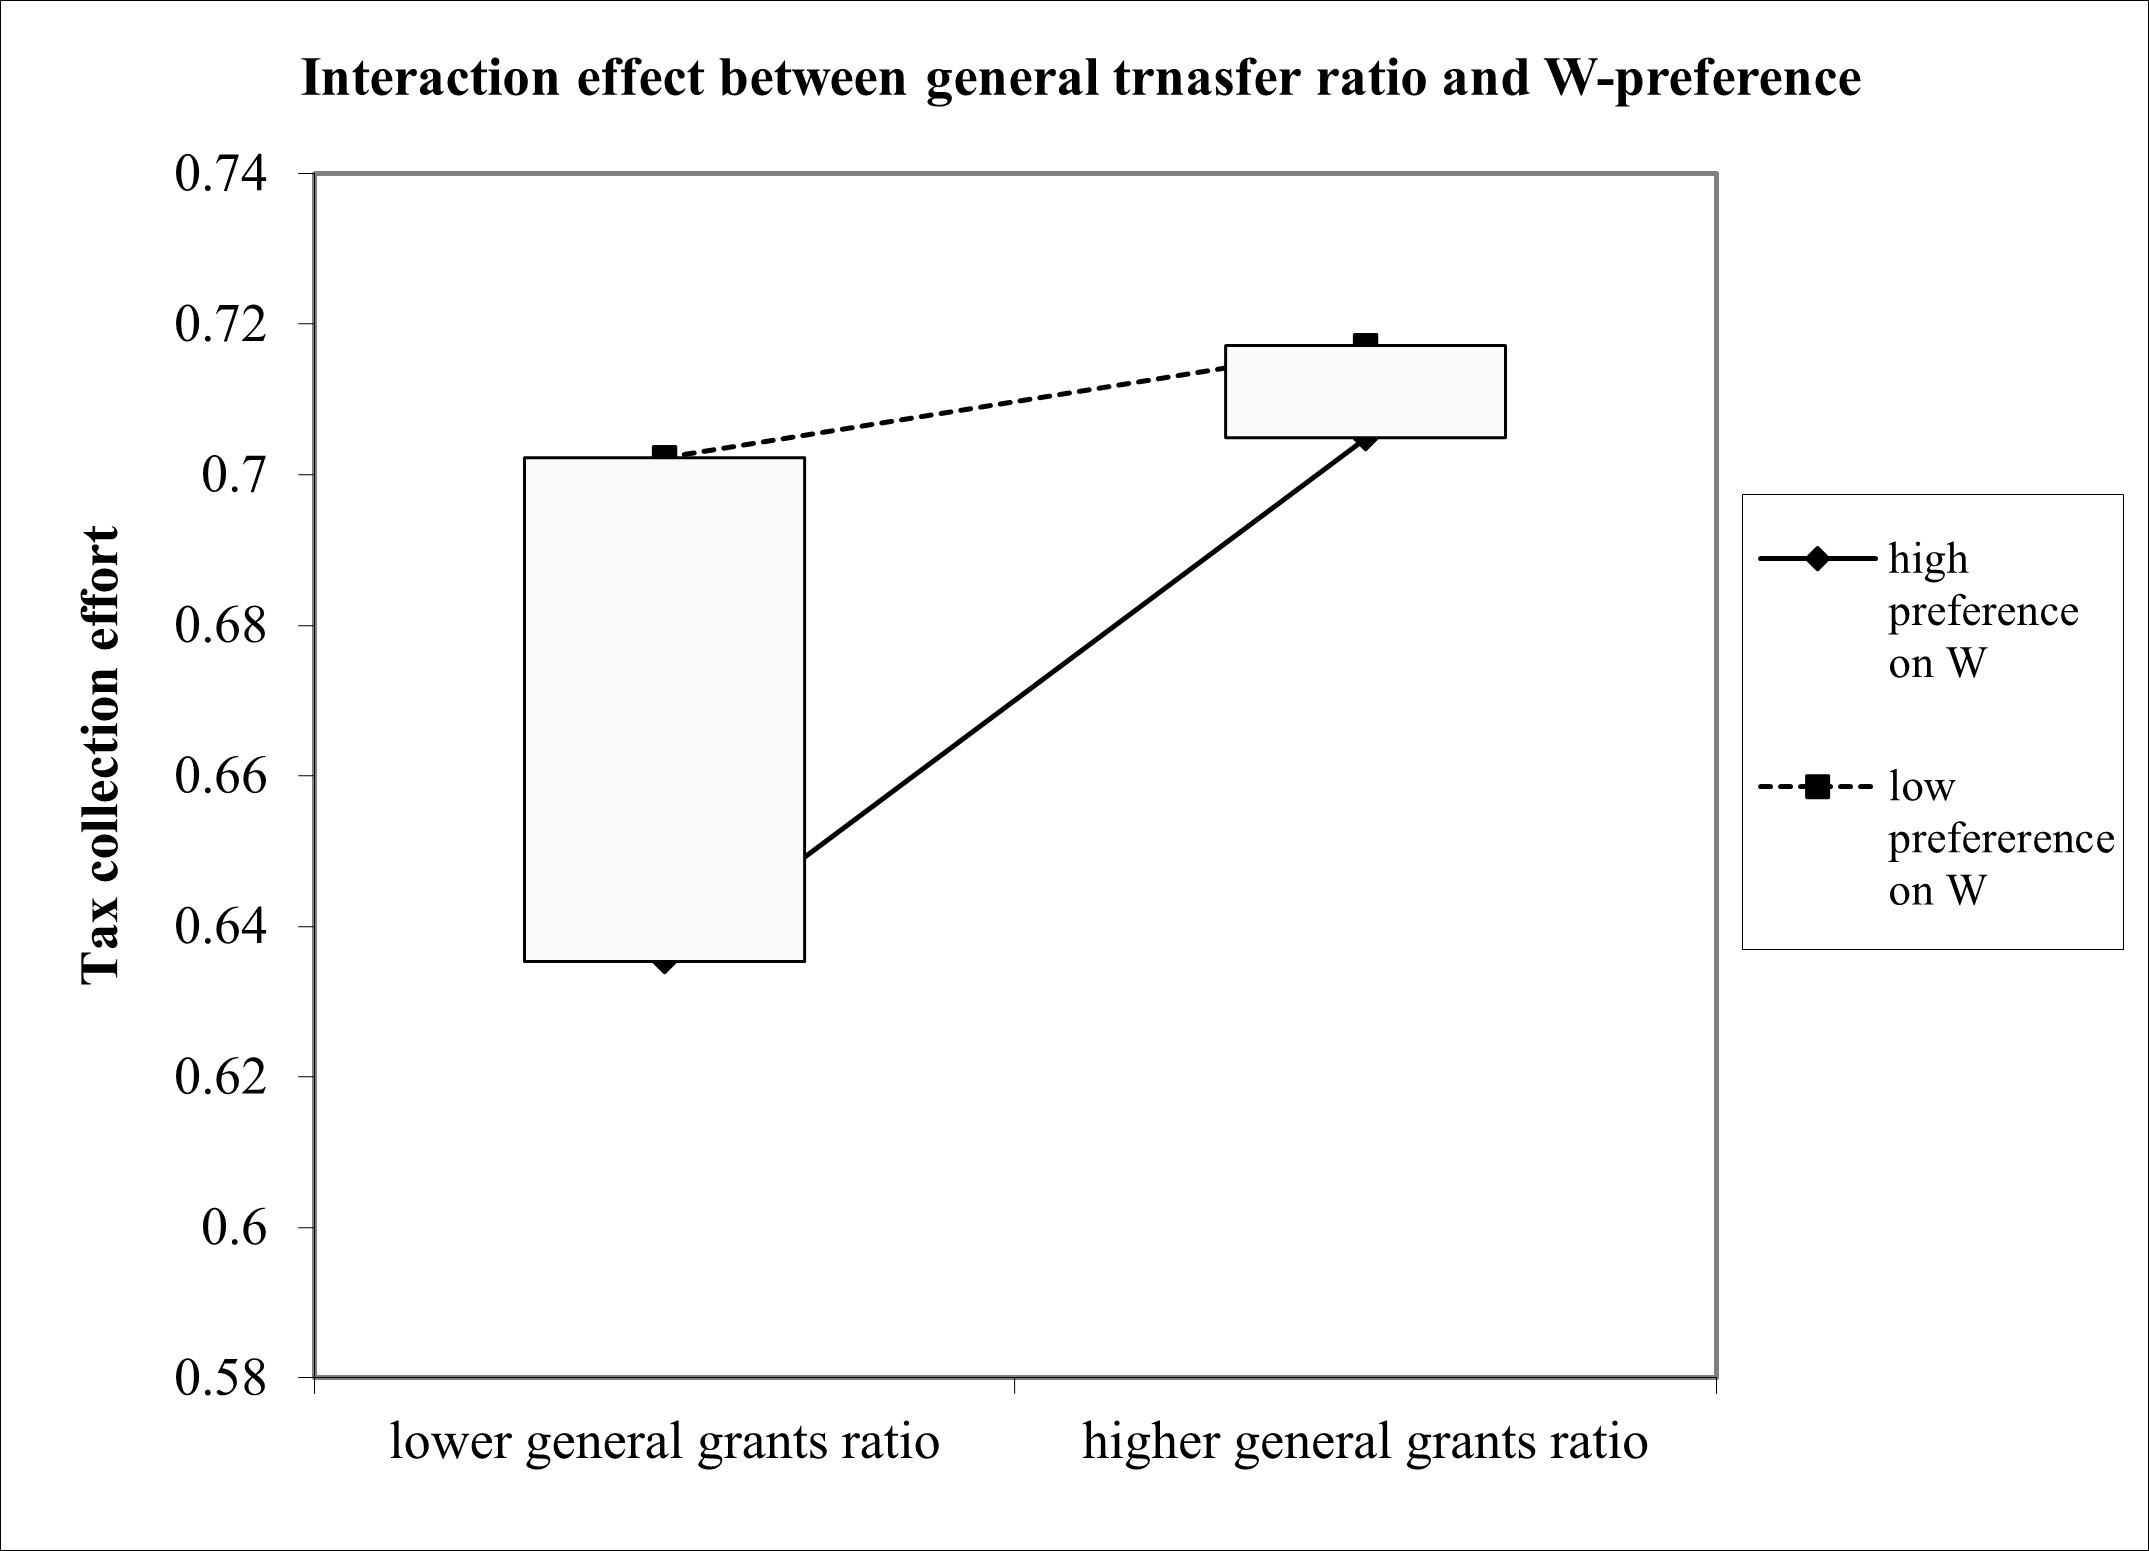
\includegraphics[scale=0.8]{Chapter-5/Figures/int_gen_W.jpg}
%     \caption[Laffer Curve for Tax Collection Effort]{Interaction effect between general trnasfer ratio and W-preference
%         \texttt{} }
%     \label{int_gen_W}
% \end{figure}

% \begin{figure}[H]
%     \centering
%     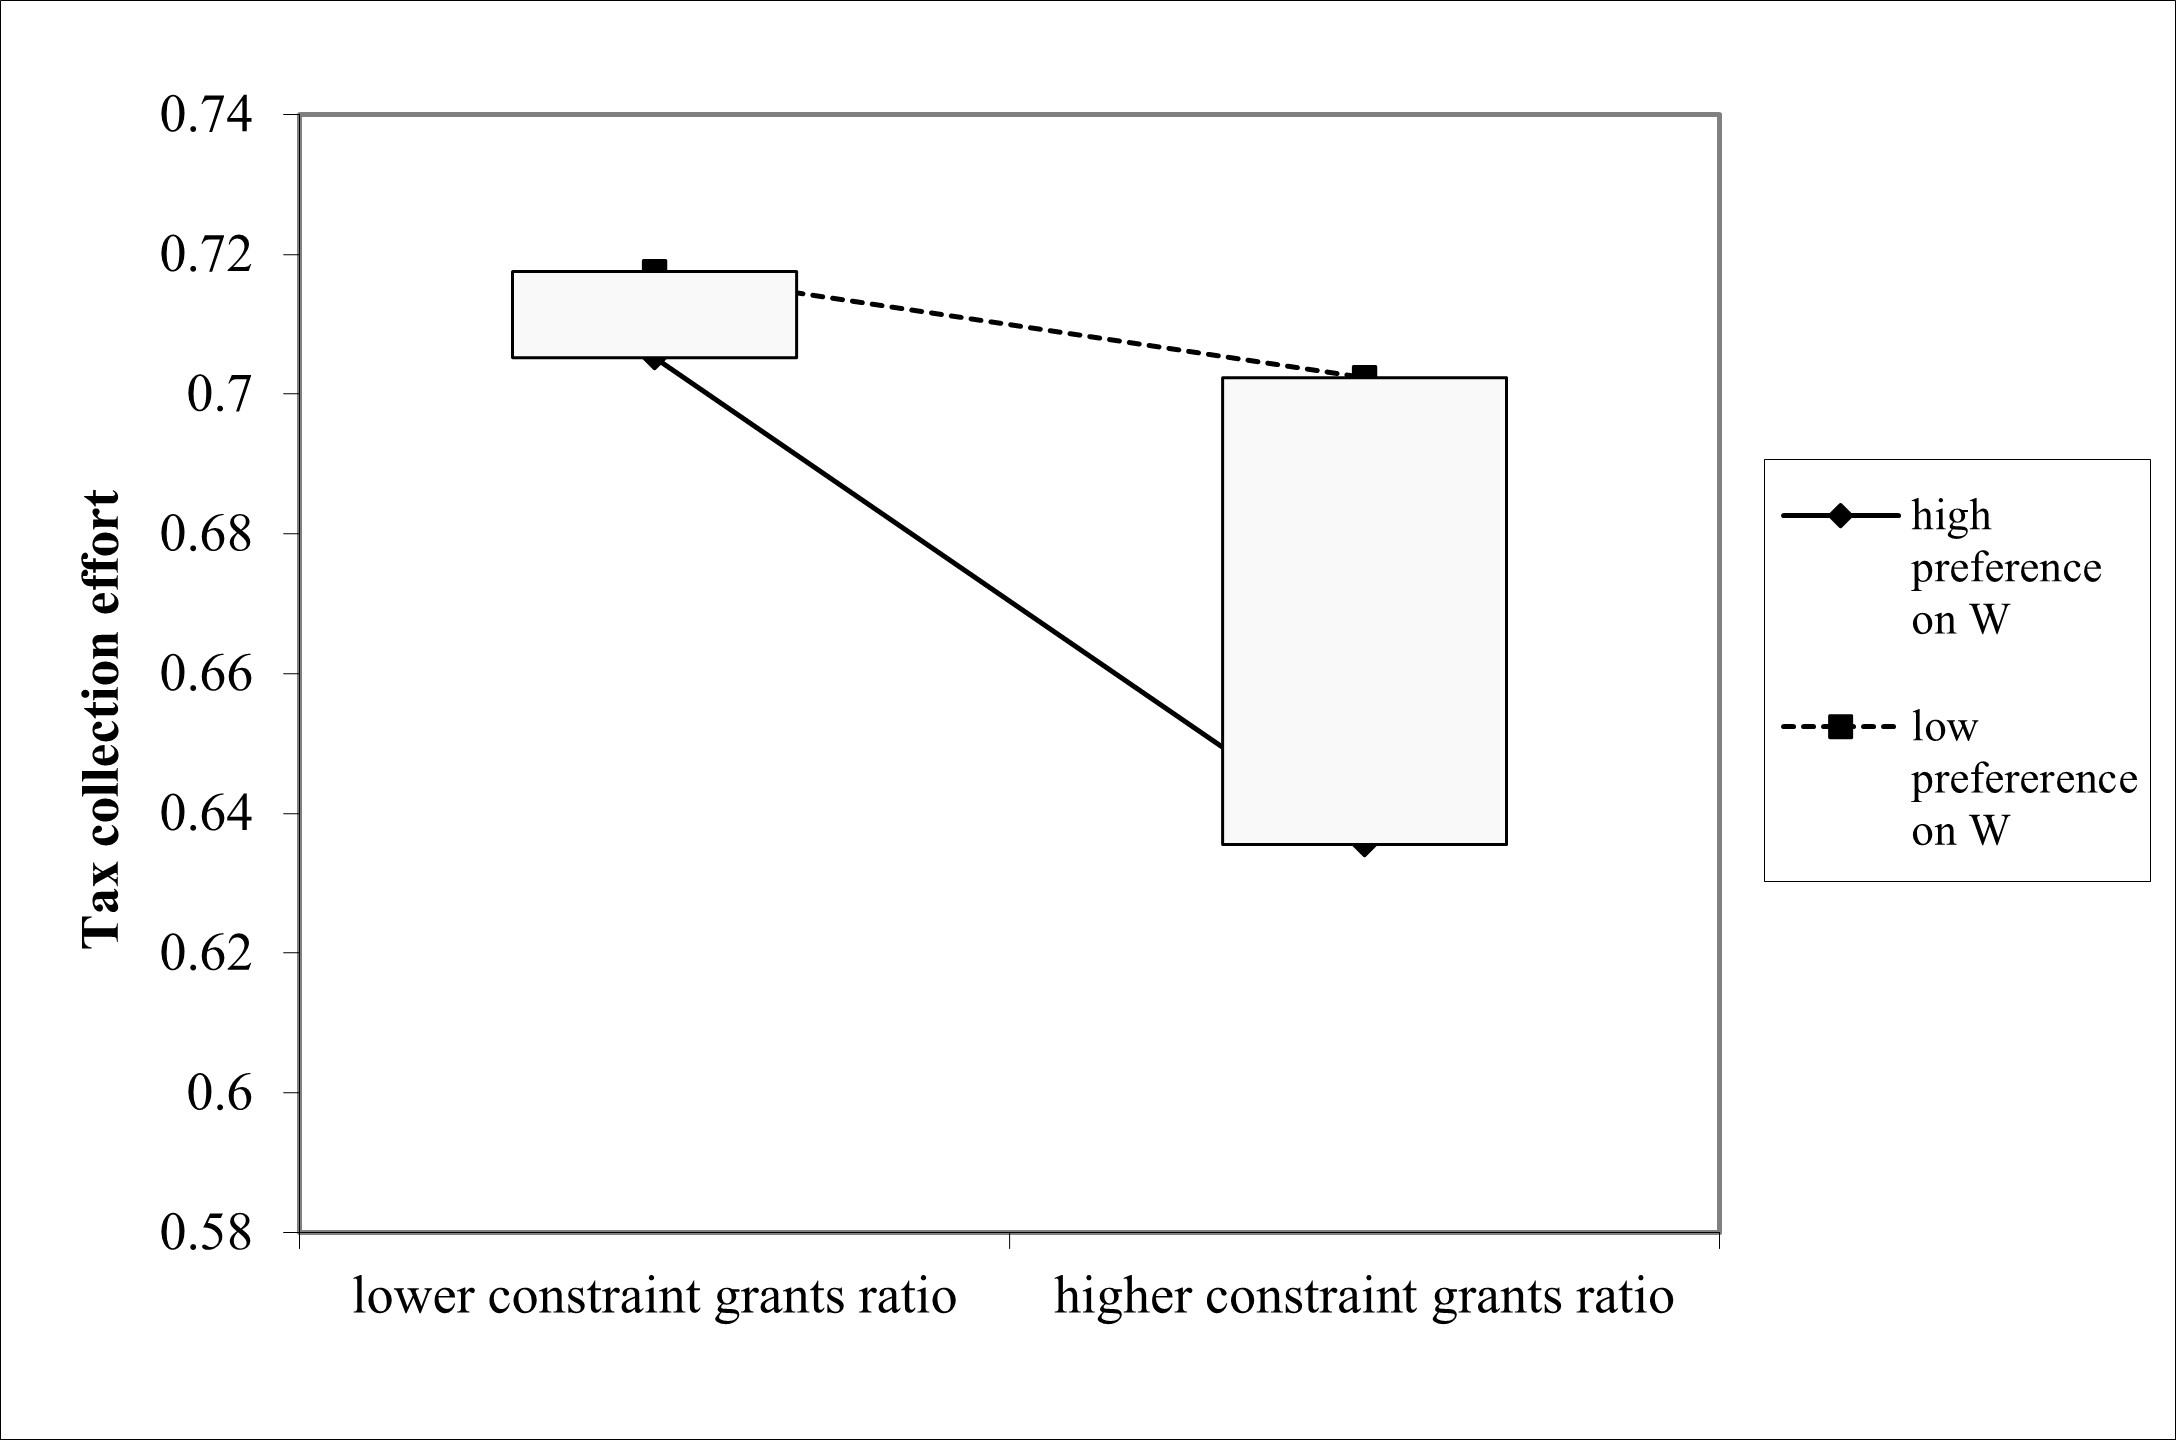
\includegraphics[scale=0.8]{Chapter-5/Figures/inter_cons_W.jpg}
%     \caption[Laffer Curve for Tax Collection Effort]{Interaction effect between welfare categorical transfer ratio and W-preference
%         \texttt{} }
%     \label{int_cons_W}
% \end{figure}

One explanation for the unexpected effect of productive categorical grants is, the effect of productive oriented grants and welfare-oriented grants could not be perfectly separated in the regression, thus the variable $constraintratio$ may not solely express productive categorical transfer. This may comes from data mixture and effect interaction. For one, we do not have an official definition about what kinds of categories of spending is considered as "productive" or "welfare". Therefore, related investigation needs to clarify the categories manually. During this process, the boundary of productive categorical transfer and welfare categorical transfer may become blurred, leading to regression results deviating from expectations. For example, \textcite{cai2005does} claims that "Infrastructure" should be interpreted broadly, including in their research that physical infrastructure (transportation, telecommunications, etc.), education, public health, and a system of well-enforced property rights and legal protections.

On the contrary, due to the relatively clear definition of general transfer payments and accurate numerical values, the econometric results align perfectly with theoretical deductions.

In addition to data mixture, another mechanism that contributes to the confounding effects of productive and welfare-specific expenditures is the diverse roles that various public investments play in economic life, which I called as interaction. For instance, social security expenditures like TANF, often perceived as purely welfare-related, also enhance the purchasing power of impoverished individuals, thereby stimulating economic growth. Similarly, public expenditures directed towards correctional facilities contribute to providing a stable and secure social environment, aiding in the reintegration of ex-convicts into society by facilitating skill development. Thus, even welfare-related expenditures may not necessarily be entirely unrelated to the overall societal output, as posited in theoretical models.


% \begin{table}[htbp]
%     \centering
%     \caption{Regression result of intergovernmental transfer on state tax collection effort}
%     \resizebox{13cm}{11cm}{
%         \begin{tabular}{ccccc}
%             \toprule
%                                         & OLS        &            & Two factors fixed effect &         \\
%             \midrule
%                                         & model-1    & model-2    & model-3                  & model-4 \\
%             \midrule
%             agrr                        & 102.6***   & 102.6***   & 19.32                    & 19.32   \\
%                                         & -15.11     & -15.11     & -1.63                    & -1.63   \\
%             minr                        & 4.513***   & 4.513***   & -2.888*                  & -2.888* \\
%                                         & -3.93      & -3.93      & (-2.20)                  & (-2.20) \\
%             manr                        & -2.163***  & -2.162***  & 0.41                     & 0.409   \\
%                                         & (-3.31)    & (-3.31)    & -0.48                    & -0.47   \\
%             infr                        & 4.669**    & 4.669**    & 1.85                     & 1.843   \\
%                                         & -2.96      & -2.96      & -0.58                    & -0.58   \\
%             fandir                      & 11.21***   & 11.21***   & 0.0485                   & 0.0543  \\
%                                         & -8.97      & -8.97      & -0.01                    & -0.02   \\
%             rer                         & 3.301***   & 3.301***   & 2.768                    & 2.766   \\
%                                         & -7.44      & -7.44      & -0.69                    & -0.68   \\
%             piepcm                      & -0.677***  & -0.677***  & -0.12                    & -0.12   \\
%                                         & (-10.67)   & (-10.67)   & (-0.89)                  & (-0.88) \\
%             mehim                       & -0.0499*** & -0.0499*** & -0.0303                  & -0.0302 \\
%                                         & (-6.14)    & (-6.14)    & (-1.28)                  & (-1.27) \\
%             unemployrate                & -0.0192*   & -0.0192*   & 0.0248                   & 0.0247  \\
%                                         & (-2.07)    & (-2.07)    & -1.59                    & -1.59   \\
%             gdppercapita                & 0.120***   & 0.120***   & 0.396                    & 0.396   \\
%                                         & -6.37      & -6.37      & -1.72                    & -1.72   \\
%             constraintratio             & -45.98*    &            & -14.38*                  &         \\
%                                         & (-2.32)    &            & (-2.56)                  &         \\
%             sw\_preference              & -9.181**   & 76.42*     & -1.806*                  & 21.61*  \\
%                                         & (-2.61)    & -2.18      & (-2.07)                  & -2.23   \\
%             int\_cons\_pref             & 70.57*     &            & 19.25*                   &         \\
%                                         & -2.22      &            & -2.22                    &         \\
%             generalratio                &            & 56.28*     &                          & 17.64*  \\
%                                         &            & -2.32      &                          & -2.57   \\
%             int\_gen\_pref              &            & -86.39*    &                          & -23.64* \\
%                                         &            & (-2.22)    &                          & (-2.23) \\
%             Constant                    & 6.760**    & -49.00*    & 2.070**                  & -15.40* \\
%                                         & -3.11      & (-2.24)    & -2.91                    & (-2.41) \\
%             \midrule
%             Observations                & 834        & 834        & 834                      & 834     \\
%             Adjusted R-sq               & 0.714      & 0.714      & 0.594                    & 0.594   \\
%             \midrule
%             t statistics in parentheses &            &            &                          &         \\
%             *p<0.05,**p<0.01,***p<0.001 &            &            &                          &         \\
%             \bottomrule
%         \end{tabular}%
%         \label{reg_igt_eff}}%
% \end{table}%


\section{Review and Summary}

This article constructs a theoretical Ramsey model based on the classification of transfer payments and the government utility function. Through solving the Ramsey model, theoretical inferences regarding the effects of general transfer and categorical transfer payments on local government tax efforts are derived. This theoretical model attempts to address two gaps in current research. Firstly, previous studies have mostly focused on discussing the impact of general transfer payments on tax efforts, with relatively fewer discussions on the role of categorical transfer, which is relatively strictly constrained. However, this article distinguishes between types of transfer payments and considers the allocation area of categorical transfer payments, thereby enabling the examination of the effects of other types of transfer payments beyond general ones. Secondly, prior research has predominantly relied on empirical tests, resulting in inconsistent conclusions on the same topic. For instance, regarding the impact of general transfer payments on tax efforts, opinions have varied between fostering and inhibiting effects. This article, through the established theoretical model, goes beyond empirical test results and discusses why the empirical evidence support divergent conclusions.

In addition to the theoretical model, this article also gathers panel data from all states in the United States from 2000 to 2019 to validate the theoretical inferences. This empirical test also innovates existing literature in two aspects. Firstly, by employing the Kalman filter, this article overcomes the difficulty of observing tax efforts and the biased proxy as substitute. Secondly, through moderating effect regression analysis, the article partially confirms the theoretical inferences.

Of course, the article also has certain limitations. Firstly, the theoretical inference regarding the impact of productive categorical transfer on tax efforts has not been empirically supported. I provided two potential reasons of the divergence, but further discussion is needed to determine whether the theoretical prediction is supported. Secondly, the article fails to provide a clear theoretical inference regarding the impact of welfare-specific transfer payments on tax efforts.

Future research in this area could focus on three main directions. Firstly, efforts could be made to improve the quality of data, particularly in accurately distinguishing between productive specific-purpose transfer payments and welfare-specific specific-purpose transfer payments during data classification. Secondly, regarding empirical testing methods, future research could explore how to accurately identify the effects of specific-purpose transfer payments in empirical tests.




% Table generated by Excel2LaTeX from sheet 'Sheet1'
% \begin{table}
%     \centering
%     \caption{Variables, measurement and data source}
%     \resizebox{\textwidth}{8cm}{
%         \begin{tabular}{c|p{11.215em}|p{6.645em}|p{6.93em}|c|c}
%             \toprule
%             \multicolumn{3}{p{24.005em}|}{Variables and Abbreviation}     & Meaning                                                       & \multicolumn{1}{p{5.715em}|}{Data Source} & \multicolumn{1}{p{5.715em}}{Time Period}                                                                                                                                                 \\
%             \midrule
%             \multicolumn{1}{c|}{\multirow{14}[28]{*}{Control Variables}}  & Agriculture                                                   & agrr                                      & \multirow{10}[20]{*}{Industrial gdp}                    & \multicolumn{1}{c|}{\multirow{10}[20]{*}{Bereau of Economic Analysis}}   & \multicolumn{1}{c}{\multirow{14}[28]{*}{2000-2019}} \\
%             \cmidrule{2-3}                                                & Mining                                                        & minr                                      & \multicolumn{1}{c|}{}                                   &                                                                          &                                                     \\
%             \cmidrule{2-3}                                                & Manufacturing                                                 & manr                                      & \multicolumn{1}{c|}{}                                   &                                                                          &                                                     \\
%             \cmidrule{2-3}                                                & Wholesale trande and Retail Trade                             & trader                                    & \multicolumn{1}{c|}{}                                   &                                                                          &                                                     \\
%             \cmidrule{2-3}                                                & Transportation and warehousing                                & tandwr                                    & \multicolumn{1}{c|}{}                                   &                                                                          &                                                     \\
%             \cmidrule{2-3}                                                & Information                                                   & infr                                      & \multicolumn{1}{c|}{}                                   &                                                                          &                                                     \\
%             \cmidrule{2-3}                                                & Finance and insurance                                         & fandir                                    & \multicolumn{1}{c|}{}                                   &                                                                          &                                                     \\
%             \cmidrule{2-3}                                                & Real estate and rental and leasing                            & rer                                       & \multicolumn{1}{c|}{}                                   &                                                                          &                                                     \\
%             \cmidrule{2-3}                                                & Health care and social assistance                             & hsr                                       & \multicolumn{1}{c|}{}                                   &                                                                          &                                                     \\
%             \cmidrule{2-3}                                                & Professional, scientific, educational, and technical services & pster                                     & \multicolumn{1}{c|}{}                                   &                                                                          &                                                     \\
%             \cmidrule{2-5}                                                & Median household income                                       & mehi                                      & \multicolumn{1}{c|}{}                                   & \multicolumn{1}{c|}{\multirow{4}[8]{*}{FRED Data Base}}                  &                                                     \\
%             \cmidrule{2-3}                                                & Unemployment rate                                             & unemployrate                              & \multicolumn{1}{c|}{}                                   &                                                                          &                                                     \\
%             \cmidrule{2-3}                                                & person income expenditure per capita                          & iepcm                                     & \multicolumn{1}{c|}{}                                   &                                                                          &                                                     \\
%             \cmidrule{2-3}                                                & GDP percapita                                                 & gdp                                       & \multicolumn{1}{c|}{}                                   &                                                                          &                                                     \\
%             \midrule
%             \multicolumn{1}{c|}{\multirow{3}[6]{*}{independent variable}} & Welfare spending preference                                   & w\_preference                             & Welfare preferernce of federal and state government     & \multicolumn{1}{c|}{\multirow{3}[6]{*}{State Expenditure Annual Report}} & \multicolumn{1}{c}{\multirow{3}[6]{*}{2000-2019}}   \\
%             \cmidrule{2-4}                                                & general ratio                                                 & gen\_ratio                                & Federal grants ratio with no constraints                &                                                                          &                                                     \\
%             \cmidrule{2-4}                                                & productive spending matching ratio                            & cons\_ratio                               & Federal categorical grants ratio on productive spending &                                                                          &                                                     \\
%             \bottomrule
%         \end{tabular}}%
%     \label{datasource}%
% \end{table}%
% % Table generated by Excel2LaTeX from sheet 'xtregionolsss0212'
